\chapter{DDoS Prevention by Multi-Agent Reinforcement Learning}\label{chap:ddos-rl}
?? Something to elaborate on versus paper: design of Ryu controller?

% \section{Threat Model}
% \section{Agent Design}
% \subsection{Weaknesses in Prior Art}
% \subsection{Feature Spaces}
% \subsection{Reward Functions}
% \subsection{Action Spaces}
% \subsection{Systems and Threat Considerations}
% \section{System Design}
% \section{Modified Learning Algorithms}
% \section{Methodology}
% \subsection{Traffic Modelling}
% \subsection{Topologies and Testing Environments}
% \section{Evaluation}
% \subsection{Congestion-aware Traffic}
% \subsection{Congestion-unaware Traffic}
% \subsection{Increased Attack Volume}
% \subsection{Computational Cost}

\section{Introduction}
Network anomaly detection and intrusion detection/prevention are continually evolving problems, compounded by the partial, non-\emph{independent and identically distributed} (IID) view of data at each point in the network.
Attacks and anomalous behaviours evolve, becoming more sophisticated or employing new vectors to harm a network or system's confidentiality, integrity, and availability without being detected \cite{DBLP:journals/comsur/BhuyanBK14}.
These attacks and anomalies have measurable consequences and symptoms which allow a skilled analyst to infer new signatures for detection by misuse-based classifiers, but unseen attacks may only be defended against after-the-fact.
This issue is inherent to \emph{misuse-} or \emph{signature-based} intrusion detectors, and it has been long-hoped that \emph{anomaly-based} detectors would surpass this by making effective use of statistical measures \cite{DBLP:journals/comsur/BhuyanBK14}.

While \emph{machine learning} (ML) approaches seem like a sensible fit for this problem, in \citeyear{DBLP:conf/sp/SommerP10} \citeauthor{DBLP:conf/sp/SommerP10} identified the `failure to launch' of ML-based anomaly detection systems---a distinct lack of real-world system deployments \cite{DBLP:conf/sp/SommerP10}.
To quite a large extent, this remains the case today.
They posit that their use is made difficult due to significant operational differences from standard ML tasks, including: the high cost of errors and extraordinarily low tolerance for false positives inherent to network intrusion detection \cite{DBLP:conf/ccs/Axelsson99}; a general lack of recent, openly available (and high-quality) training data; and diversity of network traffic across varying timescales combined with significant burstiness \cite{DBLP:journals/ccr/LelandWTW95}.
Above the aggregate level, the constant deployment of new services and protocols means that traffic is \emph{non-stationary} and displays an evolving notion of normality.
Learning is made harder still by the challenges encountered with unlabelled (often partial) data.
All of these factors greatly inflate the difficulty of the detection problem.

%?? Make it clearer here what problem I specifically want to solve: principally a particular class of DDoS attacks; volume-based DDoS attacks. Amplification attacks are just a specialisation, this can be made more obvious. I think I need to be clearer about the \emph{intended deployment environment} of service hosts (i.e., not ISPs).

For certain classes of problem e.g., volumetric \emph{distributed denial of service} (DDoS) attacks, \emph{reinforcement learning} (RL) offers another perspective.
%?? Unclear explanation of RL here?
RL agents operate by following a \emph{policy} to interact with or control a system, while at the same time using observed performance metrics and deliberate exploration to dynamically improve this policy.
In this way the role of a RL agent differs from that of a standard classifier, adaptively reacting to threats by assuming the role of a feedback loop for network optimisation, typically to safeguard service guarantees.
In a sense, this allows us to ``overcome'' some of the difficulties of the detection problem by monitoring \emph{performance characteristics and consequences} in real-time; by looking for (and controlling) the effect rather than the cause.
Long-term, we expect that the value of RL-based defence systems will be to augment what existing misuse-based solutions can provide, by automatically alerting, recording and controlling what are believed to be illegal system states.
The goal of this work is much less general; we aim to prevent volume-based DDoS attacks with the aid of RL-based techniques (an important goal in its own right), while bringing to light the flexibility and applicability of these techniques in the security domain.
%Whether it takes direct control of the network, or is used indirectly to optimise a key part of another system, more powerful `deep' RL techniques (and well-founded action spaces) aren't yet well explored for network IDS/IPS.
%These range from more modern training algorithms \cite{DBLP:journals/corr/SchulmanWDRK17, DBLP:conf/icml/SchulmanLAJM15}, to evolutionary strategies \cite{DBLP:journals/corr/SalimansHCS17, DBLP:journals/corr/abs-1802-08842}, hierarchical action composition \cite{DBLP:journals/corr/abs-1710-09767}, and competitive multi-agent learning \cite{DBLP:journals/corr/abs-1710-03748}.

To date, there have been few applications of this class of algorithms towards intrusion detection and prevention which make use of their full potential for online control, rather than using them as the basis for a classifier.
We aim to take steps to redress this and establish their proper capabilities, beyond simple ``blind application''.
%?? Expand as required
What approaches do exist are aimed towards the task of adaptive online DDoS mitigation, and rely upon learning to control probabilistic packet drop.
%?? THAT IS A MAJOR CONTRIB, MENTION IT EVERYWHERE YOU CAN

%?? Discuss the most important conclusions before the outline.
We find that the existing work for this task \cite{DBLP:journals/eaai/MalialisK15} fails to account for congestion-aware traffic (i.e., TCP) and environments with high host density per egress point, achieving poor results due to an overly coarse view of the network.
To remedy this, we make throttling decisions on a per-source basis and present the engineering decisions this mandates: updating RL agents from multiple traces per timestep, timed random sequential action computation and a supporting \emph{software-defined network} (SDN) architecture.
In tandem with the development and evaluation of an effective state space and model, we provide the design of a second model inspired by past work on algorithmic DDoS prevention, as an example of the integration of domain-specific knowledge.
Our introduction of per-source decisions improves substantially upon the state-of-the-art when acting upon most internet traffic (i.e., congestion-aware protocols), and we show that our second model achieves excellent performance for high host density in this case.
Crucially, both models remain protocol- and content-agnostic to offer future-proofing against the rollout of future protocols like QUIC \cite{DBLP:conf/sigcomm/LangleyRWVKZYKS17}.
%?? Also algorithmic enhancements such as multiple actions per timestep, 
%?? PROTOCOL-AGNOSTIC -- HOW WILL THESE THINGS COPE WITH QUIC ET AL.?!?!

\subsection{Contributions}
This paper contributes two source-level granularity approaches to RL-driven DDoS prevention (\emph{Instant} and \emph{Guarded} action models), improving upon past aggregate-based models (\cref{sec:ddos-mitigation-with-per-flow-reinforcement-learning}).
These are designed to make effective decisions irrespective of protocol, and act on individual flows at the edge of any network topology.
We offer an in-depth investigation into suitable features for automatic DDoS mitigation, with qualitative and quantitative justification (\cref{sec:rethinking-the-state-space}).
These features have been suggested by past studies, and independently tested in their own contexts.
Our study is the first attempt to quantify the individual efficacy of each in an RL setting.

We implement reactive simulations of HTTP and VoIP web-server traffic, designed to test system characteristics that packet trace playback fails to capture (\cref{sec:a-new-normal}).
To our knowledge, this is the first attempt to study or replicate Opus-based VoIP traffic, which has become commonplace since the codec's release in 2012.
These new traffic models inform an empirical evaluation of our new models against the state-of-the-art in RL-based DDoS mitigation using (\cref{sec:the-results-of-doing-so}), alongside a discussion of security concerns and real-world deployment (\cref{sec:discussion}).
We additionally compare our work against SPIFFY \cite{DBLP:conf/ndss/KangGS16}, reuniting two divergent strands of research and grounding the study of RL-based DDoS defences.

\section{Background and Threat Model}
%?? Introduce RL, related definitions etc.

\subsection{Distributed Denial of Service}
%?? DDoS attack variants (leading into characteristics, supporting features). Amplification (UDP \cite{DBLP:conf/ndss/Rossow14}, TCP \cite{DBLP:conf/uss/KuhrerHRH14}), Transit-link (Crossfire \cite{DBLP:conf/sp/KangLG13}, Coremelt \cite{DBLP:conf/esorics/StuderP09}). Mirai botnet's involvement \cite{DBLP:conf/uss/AntonakakisABBB17}.

%?? Explain amplification attack, maybe transit-link?

\emph{Distributed denial of service} (DDoS) attacks are concentrated efforts by many hosts to reduce the availability of a service, typically to inflict financial harm or as an act of vandalism.
Attackers achieve this by either exploiting peculiarities of operating system or application behaviour in \emph{semantic attacks} (e.g., \emph{SYN flooding attacks}), or overwhelming their target through sheer volume of requests or inbound packets (\emph{volume-based attacks}) \cite{DBLP:conf/imc/JonkerKKRSD17}.
Hosts often participate unwillingly, typically having been recruited into a \emph{botnet} by malware infection to be orchestrated from elsewhere \cite{DBLP:conf/uss/AntonakakisABBB17}.

Although there are variations of each class of attack, flooding attacks are the most relevant to our work.
\emph{Amplification attacks} exploit services who eagerly send large replies in response to small requests, where UDP-based services like DNS and NTP are most exploitable \cite{DBLP:conf/ndss/Rossow14, DBLP:conf/uss/KuhrerHRH14}.
Malicious hosts send many small requests, spoofed to appear as though they originated from the victim, causing many large replies to be sent to the intended target---significantly increasing a botnet's throughput while masking the identity of each participant.
\emph{Transit-link/link-flooding attacks} have been the subject of recent attention, wherein malicious traffic is forwarded across core links needed to reach a target (but not to the target itself) \cite{DBLP:conf/sp/KangLG13, DBLP:conf/esorics/StuderP09}.

% \subsection{Reinforcement Learning}\label{sec:reinforcement-learning}
% \emph{Reinforcement learning} (RL) is a variant of machine learning principally concerned with training an agent to choose an optimal sequence of actions in pursuit of a given task \cite{RL2E}.
% We assume the agent has a certain amount of knowledge whenever a decision must be made: at any point in time $t$, it knows which \emph{state} it is in ($S_t \in \mathcal{S}$), the set of \emph{actions} which are available to it ($\operatorname{A}(S_t) \subseteq \mathcal{A}$) and a numeric \emph{reward} obtained from the last action chosen ($R_t \in \mathbb{R}, A_{t-1} \in \operatorname{A}(S_{t-1})$).
% This model of system interaction is a \emph{Markov Decision Process} (MDP).
% RL methods combine this information with a current \emph{policy} $\pi$ to determine which action should be taken: such a choice need not be optimal if an agent needs to further explore some region of the state space.
% The policy is refined by updating value estimates for state-action pairs or via policy gradient methods, meaning that RL-based approaches learn adaptively and online if reward functions are available in the environment they are deployed in.
% In practice, this means that agents are able to automatically adapt to evolving problems without operator intervention or a new, custom-built training corpus.

% From any point in a sequence of decisions, we may describe the sum of rewards yet to come as the \emph{discounted return}, $G_t = R_{t+1} + \gamma R_{t+2} + \gamma^2 R_{t+3} + \ldots$, choosing the discount factor $\gamma \in [0,1)$ to determine how crucial future rewards are vis-\`{a}-vis the current state.
% Formally, an agent's goal is to choose actions which maximise the \emph{expected discounted return} $\operatorname{\mathbb{E}_{\pi}}[G_t]$.

% %?? Include some details of function approximation in the formalisation? I.e. tile coding, stability and convergence guarantees...

% There is immense variation in \emph{how} policies and/or values may be learned, reliant upon the learning environment, problem and required convergence guarantees.
% In particular, we focus on methods which choose actions according to their value estimates from the current state: let $\operatorname{q}(s, a) \in \mathbb{R}$ be the estimate of action $a$'s value if it were to be taken in state $s$.
% %?? Revisit the maths here, d, dim A, s...
% Exact (tabular) representations require that we store a value estimate for each action in every state---if state is real-valued or high-dimensional, then computation and storage quickly become infeasible.
% To cope with a continuous state and/or action space, one valuable technique is to employ linear function approximation backed by \emph{tile coding} \cite[pp.\ \numrange{217}{221}]{RL2E}.

% \begin{figure}
% 	\centering
% 	\begin{subfigure}{0.4\linewidth}
% 		\resizebox{\linewidth}{!}{
% 		\begin{tikzpicture}
% 		\node at (0,0.3){$s = \begin{pmatrix}
% 			0.7 \\
% 			0.3
% 			\end{pmatrix}$};
% 		\node at (0,-1) {$\bm{x}(s,\cdot) = \begin{Bmatrix}
% 			T_{1,9}, \\
% 			T_{2,5}, \\
% 			T_{\mathit{bias}}
% 			\end{Bmatrix}$};
		
% 		\node at (2.5,-0.5) {
% 			\begin{tikzpicture}
% 			\draw[step=0.5cm,color=uofgcobalt,opacity=0.7,shift={(0,0)},label=above:{Tiling 0}] (-0.5,-0.5) grid (1,1);
% 			\fill[uofgcobalt,opacity=0.5] (0.5,-0.5) rectangle (1,0);
% 			\node[color=uofgcobalt] at (0,1.1) {\footnotesize Tiling 1};
			
% 			\draw[step=0.5cm,color=uofgpumpkin,opacity=0.9,shift={(0.25,-0.25)},label=above:{Tiling 1}] (-0.5,-0.5) grid (1,1);
% 			\fill[uofgpumpkin,opacity=0.5,shift={(0.25,-0.25)}] (0,0) rectangle (0.5,0.5);
% 			\node[color=uofgpumpkin!50!uofgrust] at (0.25,-0.95) {\footnotesize Tiling 2};
			
% 			\node[circle, black, draw,
% 			fill, radius=0.5pt, inner sep=0pt,minimum size=1.5pt, label=above:{$s$}] at (0.625,-0.125) {};
% %			\filldraw (0.625,-0.125) circle[radius=1.5pt,label=above:{$s$}];

% 			\draw[->] (-0.25,-0.5)--(-0.25,0.85);
% 			\draw[->] (-0.25,-0.5)--(1.1,-0.5);
			
% 			\node at (1,-0.7) {\footnotesize 1};
% 			\node at (-0.4,0.75) {\footnotesize 1};
% 			\node at (-0.35,-0.6) {\footnotesize 0};
% 			\end{tikzpicture}
% 		};
		
% 		\end{tikzpicture}
% 		}
% 		\caption{Tile Coding\label{fig:tilecode-code}}
% 	\end{subfigure}%
% 	\begin{subfigure}{0.4\linewidth}
% 		\resizebox{\linewidth}{!}{
% 		\begin{tikzpicture}
% 		% Top half
% 		\def\topacs{
% 			{-0.3,-0.5,-0.1,0.8},
% 			{0.1,0.1,-0.2,0.3},
% 			{0.3,0.4,0.2,-0.4}%
% 		}
	
% 		\foreach \line [count=\y] in \topacs {
% 			\foreach \pix [count=\x] in \line {
% 				\ifthenelse{\lengthtest{\pix pt < 0 pt}}{
% 					\pgfmathtruncatemacro\lambda{(\pix+1)*100}
% 					\draw[shift={(-0.7,0)},fill=midac!\lambda!lowac] (0.7*\x,-0.35*\y) rectangle +(0.7,0.35);
% 				}{
% 					\pgfmathtruncatemacro\lambda{\pix*100}
% 					\draw[shift={(-0.7,0)},fill=highac!\lambda!midac] (0.7*\x,-0.35*\y) rectangle +(0.7,0.35);
% 				}
% 				\node[shift={(-0.35,0.175)}] at (0.7*\x,-0.35*\y) {\footnotesize \pix};
% 			}
% 		}
	
% 		\draw[xstep=0.7cm,ystep=0.35cm,shift={(0,0)}] (0,-1.06) grid (2.8,0);
% 		\node[label=left:{$T_{1,9}$},shift={(0,-0.125)}] at (0,0) {}; 
% 		\node[label=left:{$T_{2,5}$},shift={(0,-0.125)}] at (0,-0.375) {}; 
% 		\node[label=left:{$T_{\mathit{bias}}$},shift={(0,-0.125)}] at (0,-0.75) {};
		
% 		% bottom half
% 		\def\botacs{
% 			{0.1,0.0,-0.1,0.7}%
% 		}
	
% 		\foreach \line [count=\y] in \botacs {
% 			\foreach \pix [count=\x] in \line {
% 				\ifthenelse{\lengthtest{\pix pt < 0 pt}}{
% 					\pgfmathtruncatemacro\lambda{(\pix+1)*100}
% 					\draw[shift={(-0.7,-1.275)},fill=midac!\lambda!lowac] (0.7*\x,-0.35*\y) rectangle +(0.7,0.35);
% 				}{
% 					\pgfmathtruncatemacro\lambda{\pix*100}
% 					\draw[shift={(-0.7,-1.275)},fill=highac!\lambda!midac] (0.7*\x,-0.35*\y) rectangle +(0.7,0.35);
% 				}
% 				\node[shift={(-0.35,-1.1)}] at (0.7*\x,-0.35*\y) {\footnotesize \pix};
% 			}
% 		}
	
% 		\draw[xstep=0.7cm,ystep=0.35cm,shift={(0,-1.275)}] (0,-0.35) grid (2.8,0);
% 		\node[label=left:{$\mathit{Total}$},shift={(0,-0.175)}] at (0,-1.275) {};
		
% 		\draw [->] (2.45, -1.9) -- (2.45, -1.65);
% 		\end{tikzpicture}
% 		}
% 		\caption{\centering Value Estimation and Action Selection\label{fig:tilecode-select}}
% 	\end{subfigure}
	
% 	\caption{
% 		An example of tile coding for 2-dimensional state and 4 actions, using 2 tilings, 3 tiles per dimension, and a bias tile.
% 		All components of $s$ are clamped to $[0,1]$.
% 		For simplicity, we denote $\bm{x}(s,\cdot)$ as a list of indices and represent the values of all actions at each tile with a vector.
% 		(a) The state $s$ activates the bias tile and exactly one tile in each tiling.
% 		(b) The action values of active tiles are summed to produce the current value estimate for each action available in $s$---for this state, local knowledge ensures that action 4 is chosen by the greedy policy despite typically being a poor choice elsewhere.
% 		\label{fig:tilecode}
% 	}
% 	\vspace{-0.6cm}
% \end{figure}

% Tile coding is a form of feature representation which converts a state-action pair into a sparse boolean feature vector $\operatorname{\mathbf{x}}(s, a)$ by subdividing a $d$-dimensional subset of the space into a number of overlapping grids with an optional bias component.
% Each tile corresponds to an entry of $\operatorname{\mathbf{x}}(s, a)$ which is set to 1 if the state-action pair lies within it.
% \Cref{fig:tilecode-code} demonstrates the process for a 2-dimensional state space, and that the numbers of tilings and tiles per dimension control feature resolution and generalisation.
% Moreover, to capture combinatorial effects or create multi-scale representation we may combine codings by concatenating individual feature vectors.
% We may then approximate an action's value with respect to a policy parameter vector $\wvec{}$, defining some $\acval{s}{a}{\wvec{}} \approx \operatorname{q}(s, a)$:
% \begin{equation}
% %	\begin{gather}
% \acval{s}{a}{\wvec{}} = \wvec{}^{\top} \operatorname{\mathbf{x}}(s, a)
% %	\end{gather}
% \label{eqn:lin-approx}
% \end{equation}
% As each component of $\wvec{}$ is the value estimate of the corresponding tile, learning an effective policy is equivalent to learning $\wvec{}$.
% Given a learning rate $\alpha \in \mathbb{R}$ and initialising $\wvec{0}=\bm{0}$, we may continually update $\wvec{t}$ using the \emph{1-step semi-gradient Sarsa} algorithm \cite[pp.\ \numrange{243}{244}]{RL2E}:
% \begin{subequations}
% 	\begin{gather}
% 	\delta_t = R_{t+1} + \gamma \acval{S_{t+1}}{A_{t+1}}{\wvec{t}} - \acval{S_t}{A_t}{\wvec{t}},\\
% 	\bm{w}_{t+1} = \bm{w}_{t} + \alpha \delta_t \nabla{\acval{S_t}{A_t}{\wvec{t}}},
% 	\end{gather}%
% 	\label{eqn:sg-sarsa}%
% 	where $\delta_t$ is known as the \emph{temporal-difference} (TD) error, and the vector gradient $\nabla$ is taken with respect to $\wvec{}$.
% \end{subequations}

% Computing the approximate value of every available action forms the basis of a policy.
% Actions with maximal value can be chosen each time (the \emph{greedy} policy), we might modify this by taking random actions with probability $\epsilon$ to encourage early exploration (the \emph{$\epsilon$-greedy policy}), or we might use some other mechanism.
% \Cref{fig:tilecode-select} extends the prior working example to show how the value of each action is computed (and which action would be chosen by a greedy policy), combining a global estimate ($T_{\mathit{bias}}$) with knowledge particular to each state.

% \begin{figure}
% 	\centering
% 	\resizebox{0.45\linewidth}{!}{
% 		\begin{tikzpicture}		
% 		% Top half
% 		\def\startacs{
% 			{0.8},
% 			{0.3},
% 			{-0.4}%
% 		}
		
% 		\foreach \line [count=\y] in \startacs {
% 			\foreach \pix [count=\x] in \line {
% 				\ifthenelse{\lengthtest{\pix pt < 0 pt}}{
% 					\pgfmathtruncatemacro\lambda{(\pix+1)*100}
% 					\draw[shift={(-0.7,0)},fill=midac!\lambda!lowac] (0.7*\x,-0.35*\y) rectangle +(0.7,0.35);
% 				}{
% 					\pgfmathtruncatemacro\lambda{\pix*100}
% 					\draw[shift={(-0.7,0)},fill=highac!\lambda!midac] (0.7*\x,-0.35*\y) rectangle +(0.7,0.35);
% 				}
% 				\node[shift={(-0.35,0.175)}] at (0.7*\x,-0.35*\y) {\footnotesize \pix};
% 			}
% 		}
		
% 		\draw[xstep=0.7cm,ystep=0.35cm,shift={(0,0)}] (0,-1.06) grid (0.7,0);
% 		\node[label=left:{$T_{1,9}$},shift={(0,-0.125)}] at (0,0) {}; 
% 		\node[label=left:{$T_{2,5}$},shift={(0,-0.125)}] at (0,-0.375) {}; 
% 		\node[label=left:{$T_{\mathit{bias}}$},shift={(0,-0.125)}] at (0,-0.75) {};
% 		\node[label=below:{\footnotesize Action 4},shift={(0.35,-0.125)}] at (0,-0.75) {};
% 		\node[label=above:{\footnotesize $\wvec{t}$},shift={(0.35,-0.125)}] at (0,0) {};
		
% 		\def\finalacs{
% 			{0.7},
% 			{0.2},
% 			{-0.5}%
% 		}
	
% 		\foreach \line [count=\y] in \finalacs {
% 			\foreach \pix [count=\x] in \line {
% 				\ifthenelse{\lengthtest{\pix pt < 0 pt}}{
% 					\pgfmathtruncatemacro\lambda{(\pix+1)*100}
% 					\draw[shift={(2-0.7,0)},fill=midac!\lambda!lowac] (0.7*\x,-0.35*\y) rectangle +(0.7,0.35);
% 				}{
% 					\pgfmathtruncatemacro\lambda{\pix*100}
% 					\draw[shift={(2-0.7,0)},fill=highac!\lambda!midac] (0.7*\x,-0.35*\y) rectangle +(0.7,0.35);
% 				}
% 				\node[shift={(2-0.35,0.175)}] at (0.7*\x,-0.35*\y) {\footnotesize \pix};
% 			}
% 		}
		
% 		\draw[xstep=0.7cm,ystep=0.35cm,shift={(2,0)}] (0,-1.06) grid +(0.7,1.06);
% 		\node[label=below:{\footnotesize Action 4},shift={(2.35,-0.125)}] at (0,-0.75) {};
% 		\node[label=above:{\footnotesize $\wvec{t+1}$},shift={(0.35,-0.125)}] at (2,0) {};
		
% 		\draw[->] (0.9,-0.5) -- node[above] {$+ \alpha \delta_t$} (1.8,-0.5);
% 		\end{tikzpicture}
% 	}
% \vspace{-0.25cm}
% \caption{
% 	The update step for \cref{fig:tilecode}, given an observed TD error $\delta_t=-0.2$ (indicating a lower observed reward than the expected long-term value of \num{0.7}) and $\alpha=0.5$.
% 	Action 4's value is thus reduced in the tiles associated with state $s$, but remains the most likely choice; the negative $\delta_t$ may have arisen from noise in the reward signal.
% 	For illustrative purposes, we choose an unrealistically high $\alpha$ (typically, $\alpha\le0.05$ is a more reasonable choice).
% 	\label{fig:tilecode-update}
% }
% \vspace{-0.6cm}
% \end{figure}

% This combination of algorithm and coding strategy is well-optimised, if actions are discrete; this allows a particularly efficient (vectorised) implementation of the policy and update rules by storing a vector of action values for each tile.
% Action values for any state are then obtained by summing the weight vectors from all activated tiles---taking $|\mathcal{A}|(n_{\mathit{tilings}}-1)$ floating point additions per decision.
% Observing that $\nabla{\acval{s}{a}{\wvec{}}} = \operatorname{\mathbf{x}}(s, a)$, further optimisations arise by considering that a tile-coded feature vector is a binary vector of constant Hamming weight (and so is amenable to representation as an array of indices, $s_{\mathit{list}}$).
% This means that we need only perform $n_{\mathit{tilings}} + 2$ additions and \num{2} multiplications per model update:
% \begin{equation}
% \bm{w}_{t+1}[i][\operatorname{index}(A_t)] = \bm{w}_{t}[i][\operatorname{index}(A_t)] + \alpha \delta_t, \forall i \in s_{\mathit{list}}.
% \label{eqn:sg-sarsa-opt}
% \end{equation}
% \Cref{fig:tilecode-update} shows how this applies to our prior example.
% If desired we may define a state space with an arbitrary number of tiles per dimension (higher-resolution, lower generalisation), yet having constant-size state vectors and constant action computation cost ($\mathcal{O}(n_{\mathit{tilings}})$).
% Beyond this, we need not store action values for tiles which have not yet been visited, conserving memory.
% A caveat of tile coding remains, in that the value of $\alpha$ must be reduced according to the number of tilings to prevent divergence at the expense of slower learning ($\alpha \leftarrow \alpha / n_{\mathit{tilings}}$).

%?? Is this \emph{actually} just sarsa? We're using fn approx (of course), but this is fraught with its own difficulties. Is it strictly speaking correct to describe it as Sarsa at this point? It's, at the very least, 1-step semi-gradient Sarsa given that it is clearly on-policy w/ fn approx...

%\subsection{Intrusion Detection}
%Probably want to talk about NIDS/IPS,
%?? Discuss mininet? Networking terms? SDN stuff?

\subsection{Motivation}\label{sec:motivation}
%?? What makes RL a suitable method for network anomaly detection, what features are most relevant?
%?? Point I was thinking of: feedback-loop-like model allows monitoring \emph{after} an action is taken to (in theory) allow forgiveness of mistakenly punished flows. This does hinge on taking a flow-by-flow look at the state space, but if we can combine knowledge of current state (duh!), the last action taken (i.e. an indicator of our previous assessment [such as high pdrop $\implies$ bad]) then perhaps a flow which falls off identically to a legit flow can be rescued.
Moving beyond the overt benefits of choosing RL-based defences for coping with non-stationary problems, we believe that there are concrete reasons for their use here.
We have seen that for other domains in particular, misclassification is a serious problem, which can introduce \emph{collateral damage} in the context of DDoS prevention.
In theory, the feedback-loop-like model allows us to monitor flows \emph{after} an action is taken to allow forgiveness of mistakenly punished flows.
This does rely upon the ability to take a flow-by-flow view of the state space, but if we can combine knowledge of current state with the last applied action, then perhaps a flow which falls off identically to a legitimate flow can be rescued.

%Which features might be best suited to this problem?
%?? Relevant features: aggregate network state (load at various points [this has been done, of course]), flow-specific measurements (upload/download ratio when bandwidth above threshold \cite{DBLP:conf/ndss/Rossow14}, packet inter-arrival times, etc.)
Other studies suggest that there are particularly useful features which make the task of online DDoS flow identification feasible.
Aggregate network load observed at various locations suggests the overall health of a network \cite{DBLP:journals/eaai/MalialisK15}, and the ratio of correspondence between pair flows can suggest asymmetry and in many cases illegitimacy \cite{DBLP:conf/ndss/Rossow14}.
Generic volume-based statistics (counts, counts per duration, average packet sizes) have seen effectiveness in such as $k$-nearest neighbours classifiers trained to detect DDoS attacks in progress \cite{DBLP:conf/dsn/LeeKSPY17}.
Most importantly, there is evidence showing behavioural changes in response to bandwidth expansion \cite{DBLP:conf/ndss/KangGS16}, suggesting similar artefacts might arise after throttling, packet drop, or other interference.
%?? If we assume amplification attacks, we know it won't be `random' source IPs (since it's mostly-legit servers who think that they're doing a good job by replying)
%?? If we assume amplification attacks, we know it won't be `random' source IPs (since it's mostly-legit servers who think that they're doing a good job by replying)

%\section{A Plan, of Sorts}
%
%\begin{enumerate}
%	\item The main case for contribution in what I have so far:
%	\begin{itemize}
%		\item Past work reliant on unrealistic network models: tcp-like behaviour (and its effects on collateral damage) not captured, disjoint ranges of traffic distribution (no benign heavy-hitters), ISP-like topology.
%		\item I offer more realistic network emulation environment, better treatment of protocol/traffic characteristics.
%	\end{itemize}
%	\item Forthcoming: rethinking state/action spaces to operate at a finer level of granularity. New network model (live tcp back-and-forth), allows us to test collateral damage assumptions in a more realistic manner (and show clear case for moving beyond work of malialis and kudenko)
%\end{enumerate}

\subsection{Threat Model}
An attacker's goal is to minimise the fair-share bandwidth allocation that a server can give to hosts, and they are expected to act rationally in its pursuit.
Threat actors are external and act intentionally, aren't expected to be 
\emph{advanced persistent threats}, and likely range from hacktivists to moderately funded adversaries.
We assume that attacks will be volumetric DDoS attacks with the structure of an \emph{amplification attack}, and that traffic aggregates at the target (unlike in a transit-link attack).
The addresses of the set of unwitting reflector nodes are visible to the target, though any bots taking part in an attack or the machines those bots control are not revealed to the target without communication with \nth{3} party organisations such as upstream ISPs.
The discovery of any reflector by some defence system does have a cost to the attacker---there is a particularly large (yet finite) supply of viable reflector nodes \cite{DBLP:conf/ndss/Rossow14}, but the constraints that each has a large upstream bandwidth and support for high-amplification-factor protocols narrow this pool.

We do not assume that an attacker has white-box access to an agent's policy, or that they will attempt to intelligently modify flow/system state to indirectly control an agent \cite{DBLP:conf/eurosp/PapernotMJFCS16, DBLP:conf/eurosp/PapernotMSW18, DBLP:journals/corr/HuangPGDA17, DBLP:conf/sp/Carlini017}.
While they may be able to perform some degree of reverse engineering by observing the health of their own legitimate canary flows, ``stealing'' the policy through observation \cite{DBLP:conf/uss/TramerZJRR16}, investigating whether perturbations would persist in volatile network traffic statistics falls outside of the scope of this work.
The same observation extends to the possibility of poisoning attacks \cite{DBLP:journals/corr/abs-1902-09062}.
These are APT-level capabilities, whose exploration presents a rich source for future work.

\section{DDoS Mitigation with Per-flow Reinforcement Learning}\label{sec:ddos-mitigation-with-per-flow-reinforcement-learning}
Given existing works, my hypothesis here is that the best method for advancing past the current shortcomings of \gls{acr:rl}-based \gls{acr:ddos} mitigation is to design agents such that filtering decisions are computed per flow.
However, these alterations must account for computational constraints imposed by the deployment environment.
For instance, the amount of flows passing over an agent is unbounded for larger networks, potentially inflicting huge inference and monitoring costs on agents.
These require dedicated, careful handling.
I describe and justify my approach, domain-specific algorithmic improvements, and present two action models, one of which draws on domain knowledge introduced by SPIFFY~\parencite{DBLP:conf/ndss/KangGS16}.

\subsection{System design and assumptions}
A deployment environment is a network with a set of \emph{ingress/egress points} from its domain of control, through which traffic can flow, and a set of protected \emph{destination nodes}.
These nodes may be services, servers, or in the case of \glspl{acr:as} and transit networks, egress points leading to other networks.
Agents are co-located with each egress switch (i.e., $k$ ingress points from other \glspl{acr:as} require $k$ agents), all employ the same action model/design, and control the proportion of upstream packets from each external host to discard.
Each destination node $s$ has a maximum capacity on its link utilisation, $U_s$.

We assume that the deployment environment is a moderately complex \gls{acr:sdn}-capable network, because the paradigm offers features which can directly benefit \gls{acr:rl} agents acting within.
The OpenFlow protocol allows a controller (or other authorised hosts) to install complex actions, forwarding rules and logic into a switch at runtime.
For simplicity at this stage, all agents or learners run on commodity host machines.
Furthermore, networks of this kind more naturally enable the use of \gls{acr:nfv}, allowing relocation and easy installation of learners---e.g., as examined by \textcite{DBLP:journals/tnsm/JakariaRF19}.
Agents communicate with their co-hosted OpenFlow-enabled switches---running a modified version of \gls{acr:ovs}~\parencite{open-vswitch,DBLP:conf/nsdi/PfaffPKJZRGWSSA15}---to install probabilistic packet-drop rules.

This system design applies to both software-defined and traditional networks of arbitrary shape and size.
Only the ingress and egress nodes from a network need to be OpenFlow-enabled, as it is advantageous to perform filtering as close to a flow's source as possible.\sidenote{Note that, depending on the size of the target network, this needn't be a hardware OpenFlow switch. Some degree of horizontal scaling could be achieved with \gls{acr:ovs} instances. Similarly, a P4 dataplane device could fill the same niche, making the `probabilistic packet drop' primitive similarly easy to integrate.}
In a traditional network, each agent has exclusive control over its switch's tables.
In a fully software-defined network, these agents require exclusive control over the first table, forwarding legitimate packets to subsequent tables managed by the network's controller.
The main difference is that a traditional network needs this additional hardware, and does not allow an operator to dynamically determine where the ``edge'' of their network lies through \gls{acr:vnf} relocation.

\subsection{Algorithm}
To make decisions cheaply and at low latency, we use \emph{semi-gradient Sarsa with tile coding} as described in \cref{eqn:sg-sarsa} and \cref{sec:tile-code}, rather than using neural networks or more complicated function approximators.
Exploration is introduced via $\epsilon$-greedy action selection, linearly annealing $\epsilon$ to 0 over time.
Each agent has its own internal parameter vector $\wvec{}$, and agents do not share their weight vector updates with one another (but may share experience and traces with one another).

Although the choice of a classical \gls{acr:rl} method likely brings lower theoretical performance, there are significant reasons to favour such methods; these include lower latency decision-making, lower energy usage, reduced model complexity (and training time), the availability of necessary hardware, and simpler decision boundaries.
This aligns with our goal of quick online learning, and faster adaptation to aggregate changes in traffic without introducing dedicated tensor processing hardware to networks.
Simpler decision boundaries reduce the risk of overfitting and unexpected behaviour, and we expect that the simplicity of tile-based policy computation will also greatly aid interpretability of anomalous action choices.

When choosing a learning algorithm, we compared against Q-learning as well as methods based on \emph{eligibility traces} such as Watkins's $\operatorname{Q}(\lambda)$~\parencite[pp. 312--314]{RL2E} and $\operatorname{Sarsa}(\lambda)$~\parencite[p. 305]{RL2E}.
Preliminary experiments found that Sarsa offered the best performance and behaviour.

\paragraph{Action rate}
We adapt the algorithm to prioritise rapid response to changes in network state and to visit as many state-to-state transitions as possible for effective learning.
To this end, we allow agents to make many decisions per timestep.
We maintain the last state-action pair associated with each source and destination \gls{acr:ip} address, and calculate any actions for the flows which still exist.
Finally, we update $\wvec{}$ using each available trace and the reward signal from the relevant destination.
As exploration still occurs for each action, this approach reduces $\epsilon$ multiple notches every timestep.
In turn, we increase the annealing window for $\epsilon$ by a factor of \num{2.67} so as to preserve exploration over time, by accounting for the greater volume of decisions being made.

\paragraph{Per-tile updates}
While the standard formulation of \cref{eqn:sg-sarsa} updates the value of all tiles identically (by a scalar $\alpha \delta_t$), I found it more effective in this use case to compute a different temporal difference value \emph{for each tiling}.
While we make use of the sum of all tiles' action value estimates when making decisions, each tiling is updated using only its own contribution, allowing us to set $\alpha$ to a higher value without divergence.
A crucial observation is that value updates to each tile can move by different values in different directions, converging on effective estimates sooner.

\paragraph{Decision narrowings}
When learning control on the basis of a tile-coded state space from high-dimensional state, assignment of credit to individual features for each decision is difficult because all tiles have identical gradient.
To combat this, with probability $\epsilon$ an agent will mark a flow as being governed by a subset of the state space for the next \num{5} decisions.
Each agent chooses actions on that source/destination pair using one element of local state, the global state, and the bias tile---the latter two are included to strike a balance between and accuracy and correct credit assignment.

\subsection{Feature space}\label{sec:feature-space}

\begin{figure}
	\centering
	\resizebox{0.9\linewidth}{!}{
		\begin{tikzpicture}[
	texts/.style = {text=black},
	labeltexts/.style = {text=gray},
	treeline/.style = {draw=uofgburgundy},
	treenode/.style = {texts, circle, centered, fill=white, treeline},
	load/.style = {fill=uofgcobalt},
	loadline/.style = {draw=uofgcobalt, line width=0.75mm},
	loadhide/.style = {fill=uofgcobalt!40!white},
	external/.style = {fill=uofgrust},
	externalhide/.style = {fill=uofgrust!40!white},
	hideline/.style = {draw=uofgsandstone!40!white},
	hidenode/.style = {treenode, hideline},
	grow'=right
]
	\node [treenode, loadhide, label={[texts]above:Agent 1}] (mainagent) {};
	\node [treenode, loadhide, right = of mainagent] (inner0) {};
	\node [treenode, loadhide, above right = 0.2cm and 1cm of inner0] (inner1) {};
	\node [hidenode, below right = 0.2cm and 1cm of inner0] (inner2) {};
	\node [treenode, loadhide, below right = 0.2cm and 1cm of inner1] (inner3) {};
	\node [treenode, loadhide, right = of inner3] (inner4) {};
	\node [treenode, loadhide, above right = 0.2cm and 1cm of inner4, label={[texts]above:$s_0$}] (s0) {};
	\node [hidenode, below right = 0.2cm and 1cm of inner4, label={[labeltexts]above:$s_1$}] (s1) {};
	
	\node [hidenode, above left = 0.2cm and 0.5cm of inner1, label={[labeltexts]above:Agent 2}] (agent2) {};
	\node [hidenode, below left = 0.2cm and 0.5cm of inner2, label={[labeltexts]below:Agent 3}] (agent3) {};
	
	\draw[hideline, -] ($ (mainagent) + (-1,0) $) -- (mainagent);
	\draw[hideline, -] ($ (agent2) + (-1,0) $) -- (agent2);
	\draw[hideline, -] ($ (agent3) + (-1,0) $) -- (agent3);
	\draw[hideline, -] (inner1) -- (agent2);
	\draw[hideline, -] (inner2) -- (agent3);
	
	\draw[loadline, -] (mainagent) -- (inner0);
	\draw[loadline, -] (inner0) -- (inner1);
	\draw[hideline, -] (inner0) -- (inner2);
	\draw[-] (inner1) -- (inner3);
	\draw[hideline, -] (inner2) -- (inner3);
	\draw[loadline, -] (inner3) -- (inner4);
	\draw[loadline, -] (inner4) -- node [texts, above] {$U_{s_0}$} (s0) ;
	\draw[hideline, -] (inner4) -- node [labeltexts, below] {$U_{s_1}$} (s1);
\end{tikzpicture}
	}
	\caption[Global state selection for a flow across a monitored AS.]{
		Global state selection for a flow between an external host and server $s_0$ which passes over Agent 1.
		All nodes in the path taken through the defended network are filled in blue, and all link load measurements which are chosen for action computation are indicated with a thick blue line.
		\label{fig:global-state-path}
	}
\end{figure}

Our state space combines elements of global state, network link load observations as used in past work such as Marl~\parencite{DBLP:journals/eaai/MalialisK15}, with per-flow measurements.
Each is tile-coded with \num{8} tilings and \num{6} tiles per dimension, using the windows described in \cref{tab:codings}.

%?? How is global state acquired? See \cref{fig:global-state-path}. Why take paths in the way that we do? Mention deterministic ECMP routing etc...
Global state is a vector of load values in $\mathbb{R}^4$ (\unit{\mega\bit\per\second}) depending upon the bandwidth measurements regularly received from monitors in the environment.
For any flow, an agent first computes the path it would take through the network.
The incoming link utilisations of the first hop, last hop, and tertiles of the path are then tile-coded together, giving a fixed-size representation of network characteristics along the traffic path.
In the event that the path from an agent to its destination is shorter than \num{4} hops, we simply duplicate the load measurement of a middle hop or the last hop (in order of preference).
\Cref{fig:global-state-path} illustrates the process.

Global state is built in this way to offer compatibility with multipath, multi-destination networks, offering support for diverse deployment environments from endpoint servers to transit \glspl{acr:as}.
Computing the path from agent to destination is not computationally expensive.
Multipath routing is often fast since typical \gls{acr:ecmp} algorithms simply hash a packet's flow key, and are deterministic to provide consistent quality-of-service to hosts.\sidenote{It's expected that most deterministic load balancing schemes should be trivial for hosts or controller machines to compute given up-to-date topology information. More dynamic schemes which balance adaptively on a flowlet or per-packet model are somewhat out of scope---this might be captured by an expectation in link loads over all valid paths.}

%?? Path computation fast and efficient due to deterministic routing based on hashes (ECMP)
%?? Works for any arbitrary topology, even 

Each of the per-flow features included in the state vector are described and analysed throughout \cref{sec:rethinking-the-state-space}.
Each feature is tiled separately, with the exception of packet in/out count (per-window and total), mean in/out packet size, and $\Delta$ in/out rate, which are combined with the last action taken.
Rather than having the network push the data to an agent, the agent requests this information about active flows periodically to isolate it from non-control-plane traffic and to eliminate the risk of resource exhaustion by excessive requests.

\subsection{Reward function}

%?? Say ``we take $R_G$ from M and K''.
%
%?? Reward at each destination.

\newcommand{\arrload}[2]{\operatorname{load}^{#2}_{t}(#1)}
\newcommand{\uload}[1]{\arrload{#1}{\uparrow}}
\newcommand{\dload}[1]{\arrload{#1}{\downarrow}}
\newcommand{\bload}[1]{\arrload{#1}{\updownarrow}}
\newcommand{\cond}[2]{\operatorname{c}_{#1,t}#2}
%\fakepara{Reward function directionality}
%The reward functions, as defined, do not take traffic direction into account.
%We redefine these to identify overload states using both upstream and downstream loads, while allowing customisation of which direction is chosen for protection.
Every timestep $t$, each destination node $s$ generates a reward signal $R_{s,t}$.
Assume, for now, that each destination has access to some classification function $g(\cdot)$ which estimates the volume of legitimate traffic received, and expects to receive $\mathit{traffic}_s$.
Denoting the upstream, downstream, and combined loads as $\uload{s}, \dload{s}, \bload{s}$ at this node:

\begin{subequations}
	\newcommand{\load}[1]{\operatorname{load}_{t}(#1)}
	\begin{gather}
	\cond{s} = [\max(\uload{s}, \dload{s}) > U_s],\\
	R_{s,t} = (1 - \cond{s}) \frac{g(\arrload{s}{-})}{\mathit{traffic}_s} - \cond{s},\label{eqn:reward-rtx}
	\end{gather}
	replacing $\arrload{s}{-}$ in \cref{eqn:reward} with whichever load direction is prioritised according to the traffic characteristics of the deployment environment. $\cond{s}$ represents an `overloaded' condition at destination $s$, equalling 1 if either load for $s$ is greater than its capacity.\label{eqn:reward}
\end{subequations}
We choose $\uload{\cdot}$ for defending \gls{acr:udp}-based models and $\dload{\cdot}$ for \gls{acr:http} traffic, though $\bload{\cdot}$ would likely be the most suitable for general deployment or heterogeneous traffic patterns.
These choices reflect where the bulk of transmitted bytes in each traffic model are observed---and the lack of this knowledge in the general case.

While the use and definition of $g(\cdot)$ appears nebulous, there are many possible ways to infer this quantity in practice.
End-host servers may use canary flows or other active measurements, or employ existing quality-of-experience metrics in the case of \gls{acr:voip} services such as lost packets, reorderings, and jitter.
\glspl{acr:as} and transit networks may make use of reports received from downstream networks, e.g., over the \gls{acr:dots} protocol~\parencite{ietf-dots-use-cases-17}.
Even if such heuristics or perfect knowledge aren't available in deployment, a sufficiently well-trained agent needs only to greedily follow the policy it has learnt from training, allowing pre-training by a simulated environment (with perfect knowledge) to transfer to reality.

If a network is believed to be vulnerable to indirect attacks, such as link-flooding attacks, we may use the following reward:
\begin{equation}
	R_{s,t}^{\mathit{Cross}}(\beta) = \beta R_{s,t} + (1 - \beta) \min{\{R_{s',t}~|~s' \ne s\}} \label{eqn:lfa-reward}
\end{equation}
where the collaboration parameter $\beta \in [0,1]$ models the expected degree of interference between flows, and $s, s'$ are protected destination nodes in the network.
The key insight underpinning \glspl{acr:lfa} is that flows can affect a target \emph{without communicating with that target}.
$\beta$ then acts as a tunable parameter which can incentivise agents to remove flows which harm overall system health, by including the performance of the worst-performing destination.
However, such attacks (and the effectiveness of $R_{s,t}^{\mathit{Cross}}$) are not examined by this work.

\subsection{Action space}\label{sec:ddos-action-space-risks}
When monitoring a source-destination pair, an agent uses its state vector to decide which proportion of that flow's \emph{inbound} traffic should be dropped.
%?? Why pdrop? Allows for discrete action space, don't have to account for buckets/fairness/burstiness.
This is implemented by installing an action via OpenFlow, instructing its host switch to drop each relevant packet with probability $p$.
Although it invites risks which I describe shortly, agents choose to drop packets rather than impose traffic limits as it offers a discrete action space without prior knowledge of traffic characteristics or measurement.
Furthermore, we need not consider burstiness, fairness, or tuning of queue parameters (such as per-flow bucket sizes) which could limit scalability.
I present two models on how to choose $p$: \emph{Instant} agents which directly choose $p$ over s uniform domain, and \emph{Guarded} agents which follow a reduced action set controlling an \gls{acr:fsm}.

\paragraph{Instant control}
Each agent directly chooses $p \in \left\{ 0.0, 0.1, \ldots, 0.9 \right\}$, giving a discrete, static action set which cannot completely filter traffic.
These choices ensure that the rate reduction imposed on traffic from a given source \gls{acr:ip} may never be permanent or irreversible.
Since this model needs no forward planning, we found it best to set the discount factor $\gamma=0$ (making agents purely myopic).

\paragraph{Guarded control}
The measurements of \textcite{DBLP:conf/ndss/KangGS16} suggest that bot attack flows cannot scale up to match an increase in available bandwidth.
I apply their observations within the \gls{acr:rl} paradigm by constraining how an agent treats each flow using a simple \gls{acr:fsm}: we restrict $p \in \left\{ 0.00, 0.05, 0.25, 0.50, 1.0 \right\}$.
The action set is then simply to \emph{maintain}, \emph{increase}, or \emph{decrease} $p$ for a flow in single steps.
We choose these potential values for $p$ to add complete filtering to a steady progression of rate-limiters (\qty{25}{\percent} increments for congestion-unaware \gls{acr:udp} traffic).
The outlier, $p=0.05$, corresponds to roughly a \qty{50}{\percent} rate reduction for congestion-aware \gls{acr:tcp} flows in our test topology.
This uneven spread of choices for $p$ allows light and heavy rate reduction to be applied to both congestion-aware and congestion-unaware traffic as required.

To enable temporary bandwidth expansion in all deployments, every flow is initially placed under significant (but still somewhat usable) packet drop ($p=0.05$); this is chosen above the equivalent for \gls{acr:udp} due to \gls{acr:tcp}'s higher prevalence.
Most importantly, an agent must now choose to punish a flow multiple times in succession to cause rapid degradation, reducing variance while allowing an agent to see how a host reacts to structured changes in the environment.

As each agent now requires the capability to plan ahead, we require a discount factor $\gamma \ne 0$, allowing the value of future states to influence state-action value updates.
Setting $\gamma = 0.8$ was found to be the most effective choice for this hyperparameter during exploratory testing.

\paragraph{Risks}
This mode of action means that each agent is in control of pushback~\parencite{DBLP:journals/ccr/MahajanBFIPS02a}, and so carries a risk of introducing collateral damage into the network.
%This is particularly severe when handling~\gls{acr:tcp} traffic: the Mathis equation~\parencite{DBLP:journals/ccr/MathisSMO97} states that \gls{acr:tcp} bandwidth is proportional to $1/\sqrt{p}$ (noting that $p$ is nonzero in any real network) while \gls{acr:cbr} \gls{acr:udp} traffic is proportional to $1 - p$.
%%It's worth noting that there are various ways that this could be implemented, and that the application of \emph{programmable data planes} to this end are suggested as future work.
%This weakness is still present in modern TCP flavours, such as TCP Cubic which in turn has bandwidth proportional to $1/p^{0.75}$ \cite{rfc8312}.
Recall from the critical analysis of \emph{Marl} in \cref{sec:ddn-uses-security} that benign congestion-aware traffic which responds to packet loss as a congestion signal will \emph{explicitly slow down further}.
This is of particular importance due to the prevalence of \gls{acr:tcp} and other congestion-aware protocols within the Internet.
Analysis of the \gls{acr:caida} datasets for 2018~\parencite{caida-2018-passive} shows that congestion-aware traffic makes up at least \qtyrange{73}{82}{\percent} of packets, corresponding to \qtyrange{77}{84}{\percent} of data volume (\cref{adx:caida-traffic}).
The QUIC transport protocol, which has become commonplace,is congestion-aware and makes up around \qtyrange{2.6}{9.1}{\percent} of traffic observed on backbone links, depending on location and typical workload~\parencite{DBLP:conf/pam/RuthPDH18}.
%As far as future network protocols are concerned, QUIC \cite{DBLP:conf/sigcomm/LangleyRWVKZYKS17}, a congestion-aware stream transmission protocol, will behave much like TCP, showing the importance of further development to properly handle traffic with such characteristics.
Making the wrong action choices here will have a greater impact on most legitimate traffic.

Choosing the wrong granularity to apply actions can be similarly disastrous.
The other key weakness of Marl is that actions are applied on a per-switch basis.
%?? Make more sane. This is about ``Why go per-flow?''
This further justifies our focus on per-flow decisions---real-world deployments see many flows pass over any egress point, making such global actions more likely to inflict collateral damage.
%This manifests in two ways: the best-achievable performance drops, and so too does the learning rate.
We can show analytically that the intuition that per-flow decisions provide better service to carried traffic in this case.
Given the probability that a host is legitimate, $P_G \in [0,1]$, it follows that a host will be malicious with probability $P_B = 1 - P_G$.
Defining \emph{imperfect service} to mean any case where all $n$ hosts whose traffic is carried by a single switch do not share the same classification (i.e., a mixture of benign and malicious hosts), then the probability that a switch is delivering imperfect service is $P_{M,n} = 1 - (P_G^n + P_B^n)$.
\begin{thm}
	As the host-to-learner ratio $n$ increases, it is more likely that a throttling switch will exhibit imperfect service: $\forall n \in \mathbb{Z}^{+}, P_{M,n} \le P_{M,n+1}$.
\end{thm}
\begin{proof}
	\emph{Base case:} $P_{M,1}=0, P_{M,2} = 1 - P_G^2 - P_B^2 > 0$.
	
	\emph{Inductive step:} Assume that the theorem holds for $n$. Observe that $P_G^n \ge P_G^{n+1}$ (resp.\ $P_B$). It then follows that:
	\begin{align*}
	P_G^n + P_B^n &\ge P_G^{n+1} + P_B^{n+1}\\
	1 - (P_G^n + P_B^n) &\le 1 - (P_G^{n+1} + P_B^{n+1})\\
	P_{M,n} &\le P_{M,n+1} \qedhere
	\end{align*}
\end{proof}
\begin{corr}
	Restricting $P_G \in (0,1)$ so that both $P_G$ and $P_B$ are non-zero ensures strict inequality: $P_{M,n} < P_{M,n+1}$.
\end{corr}
When considering that many hosts have an especially adverse reaction to our main means of control, flow-level granularity becomes an obvious choice.

\subsection{Systems considerations}\label{sec:systems-considerations}
%Taking many actions per timestep means that any agents are assigned a larger, and potentially unbounded, set of tasks to perform every time they receive load and flow statistics from the network and their parent switch.
%This introduces some potential issues: the inability to respond to unexpected changes in flow state, delayed service of new flows, and risks that flow states become outdated.
%At their worst, these risks present additional attack surface to an adversary.
%To adapt to these problems, we must make use of \gls{acr:trs} updates.
%
%Each agent begins with an empty work list.
%For the set of flows active in any timestep, we shuffle the list and perform as many action calculations and updates as possible, within a set time limit.
%Uncompleted work is passed on to the next timestep, until the list is emptied, at which point it is repopulated using the set of available measurements.
%To ensure that flow control actions are made with recent information, we combine state vectors for unvisited flows in the current work set, and replace the stored vector for all others.
%State vector combination is done by summing deltas and packet counts, updating means via weighted sums, and replacing all other fields.
%Following the observations of \Textcite{DBLP:conf/sigcomm/ChenL0L18} concerning short flows, we maintain a deadline of \qty{1}{\milli\second}---in tests, an agent is typically able to process around \num{3} flows in this time.
%Ideally, this should be tuned based on the frequency at which statistics arrive.
%Naturally, an agent must carry work forward (and coalesce state updates) when \emph{host density} is $n>3$ (\cref{sec:ddos-evaluation}); this behaviour is not explicitly a property of network size, but relates to the cost of inference and learning.
%
%?? Hmm??

Acting on an unbounded set of flows in each timestep introduces potential issues: the inability to respond to unexpected changes in flow state, delayed service of new flows, and the risk that flow states become outdated.
At their worst, these risks present additional attack surface to an adversary.
To tackle these problems, we make use of \gls{acr:trs} updates.

The scheduler begins with a shuffled work list of active flows.
When requested, the scheduler estimates the cost of an action computation using the timing information from past inference, and proceeds down the list to send a set of flow 5-tuples to the core which can be handled in a set time limit.
The scheduler continues until the list is empty, at which point it is repopulated and reshuffled with active flows.

%Following \citeauthor{DBLP:conf/sigcomm/ChenL0L18}'s observations on handling short flows \cite{DBLP:conf/sigcomm/ChenL0L18}, we maintain a deadline of \SI{1}{\milli\second}---an agent is typically able to process around 3 flows in this time.
Following the observations of \Textcite{DBLP:conf/sigcomm/ChenL0L18} concerning short flows, we maintain a deadline of \qty{1}{\milli\second}---in tests, an agent is typically able to process around \num{3} flows in this time.
Ideally, deadlines should be tuned based on the frequency at which statistics arrive.
Naturally, an agent must carry work forward (and coalesce state updates) when \emph{host density} is $n>3$ (\cref{sec:ddos-evaluation}); this behaviour is not explicitly a property of network size, but relates to the cost of inference and learning.
The amount of processed flows per deadline depends on the agent design (required \gls{acr:fpu} operations, policy size), but also on the amount of flow telemetry data needing processed---the current implementation is written in Python, restricting this handling to a single thread.
An implementation in a systems language such as Rust or C++ would allow faster concurrent processing.

There is a risk that so much work can be queued up that an agent is never able to act on some attack flows.
A solution is to impose an upper bound on the amount of action computations/policy updates that can be performed before the work list is regenerated.
This removes the guarantee that all flows will be visited often, but if updates occur regularly then this sampling may be sufficient to achieve good performance.

\section{System Architecture}\label{sec:system-architecture}
%?? Here is where I would put my ramblings about system architecture...
We present our design of a system which supports the effective real-world deployment of RL-based DDoS mitigation.
\Cref{fig:sys-arch} displays this, separating system elements which are local to each agent from those which reside elsewhere in the network.
We operate each agent as a \emph{virtualised Network Function} (vNF) adjacent to a software-defined switch.
SDN allows a controller (or authorised hosts) to install actions, forwarding rules and logic into a switch at runtime.
Moreover, networks of this kind more naturally enable the future relocation and easy installation of learners.
Agent vNFs communicate with these co-hosted switches to install probabilistic packet-drop rules.
We describe the main purpose and operation of each module within an agent's vNF, and discuss techniques to make deployment more efficient using existing technologies.

\subsection{Core and RL Executor}\label{sec:core-and-rl-executor}
The core module is the main loop in an agent's architecture.
At each timestep, the core receives information about which flows have arrived and should be acted upon from the \emph{TRS Scheduler}.
The core then retrieves the current and previous state vector associated with each flow from the \emph{Flowstate Database}, passing them into the RL algorithm alongside the last action chosen for that flow (if available).

The RL algorithm then returns an action.
Each action is passed to the database, which computes and returns a packet drop rate according to the agent model (\emph{Instant/Guarded}) while updating flow state.
This is then converted into an OpenFlow message carrying packet drop rules; these are batched to the agent's switch using the same groupings produced by the scheduler.
Finally, timing information is passed back into the scheduler to refine its estimates about how much work should be scheduled in the next timestep.

State space sizes guarantee that an \emph{Instant} policy remains under \SI{520}{\kibi\byte}, though our sparse representation typically leads to far smaller policies: $\sim$\SI{17.8}{\kibi\byte} from our experiments.
\emph{Guarded} policies are \SI{30}{\percent} of this size.
As described earlier, action updates require a constant number of floating point operations---\num{160} floating point additions and \num{32} multiplications per update of $\wvec{}$ with per-tile updates, with \num{160} additions required to choose an action.
The vast majority of these operations can be vectorised.
Action computation for \emph{Guarded} agents is cheaper still, requiring only \num{48} additions per action.

\subsection{Stats API and Collectors}
Agents require information from the network and one another to be effective.
Our agents can act either independently, having no agent-to-agent communication, or cooperatively.
In the latter case agents transfer, when possible, \emph{experience} to one another---lists of state-action-state transitions with associated rewards.
It's noted that a transition may be high-value or surprising to one agent, while well-known to another, causing each to produce different policy updates from the same unit of experience.
For this reason we do not transfer policy deltas between agents, causing each to learn its own policy.
Which scheme achieves better performance is left to future work.

%?? How do stats get from switcehs to the agent?
Load collectors and estimators periodically push observations to each active agent vNF.
In our current implementation, load statistics are gathered via vNFs active at each network switch, though we expect that OpenFlow stats requests, NetFlow or SNMP data may be used to derive these cheaply.
Transferring state to agents and experience sharing can both be made more efficient through effective use of broadcast addressing in a target network.
Depending on the capabilities of switches in the network, the estimator can either send benign traffic estimates or parameters for use in a reward function.

Gathering and transmission of load/flow statistics would be difficult to perform quite as often as an emulated environment allows.
However, the measurements acquired in such a scenario are likely to be less noisy (by being collected over longer periods of time), which could aid effective training.

\subsection{Flowstate Database}
For each flow 5-tuple, we hold two state vectors containing the features described in \cref{sec:feature-space}---the current state, and the state which induced the last action.
To ensure that flow control actions are made with recent information, we combine state vectors for unvisited flows in the current work set.
State vector combination is done by summing deltas and packet counts, updating means via weighted sums, and replacing all other fields with the newest measurements.
For flows outside of the current work list, we simply replace the stored vector.

\subsection{TRS Scheduler}
Acting on an unbounded set of flows in each timestep introduces potential issues: the inability to respond to unexpected changes in flow state, delayed service of new flows, and the risk that flow states become outdated.
At their worst, these risks present additional attack surface to an adversary.
To tackle these problems, we make use of \emph{Timed Random Sequential} updates.

The scheduler begins with a shuffled work list of active flows.
When requested, the scheduler estimates the cost of an action computation using the timing information received from the core, proceeding down the list to send a set of 5-tuples to the core which can be handled in a set time limit.
The scheduler continues until the list is empty, at which point it is repopulated and reshuffled with active flows.

Following \citeauthor{DBLP:conf/sigcomm/ChenL0L18}'s observations on handling short flows \cite{DBLP:conf/sigcomm/ChenL0L18}, we maintain a deadline of \SI{1}{\milli\second}---an agent is typically able to process around 3 flows in this time.
We expect deadlines should be tuned based on the frequency at which statistics arrive.
The amount of processed flows per deadline depends on the agent design (FLOP count, policy size), but also on the amount of flow telemetry data needing processed---our current implementation is written in python, restricting this handling to a single thread.
An implementation in a systems language such as Rust or C++ would allow faster concurrent processing.

There is a risk that so much work can be queued up that an agent is never able to act on some attack flows.
A solution is to impose an upper bound on the amount of action computations/policy updates that can be performed before the work list is regenerated.
This removes the guarantee that all flows will be visited often, but if updates occur regularly then this sampling may be sufficient to achieve good performance.

\subsection{Agent Switches}
%?? How do we do stat collection?
Our agent switches operate a modified version of Open vSwitch, implementing an action which requests that each matched packet be dropped with a certain probability.
To get around the lack of floating-point support in many environments, we represent this probability using a 32-bit unsigned integer (scaling \num{1.0} to $2^{32}-1$).
On commodity hardware, we believe that a similar effect can be achieved using OpenFlow meters (at the expense of these being stateful measures).

We use OpenFlow groups to simplify control messages: premade tables with permitted levels of packet drop.
This saves some overhead compared to using experimenter/extension headers.
Flows are automatically given a group with the default level of packet drop (according to the chosen agent design), meaning that switches don't need to refer to a controller or the agent vNF.

%?? What do our modifications to openflow look like? How do we get around the lack of floating point math?

\begin{figure}
	\centering
	\resizebox{0.8\linewidth}{!}{\begin{tikzpicture}
		\node(remote){Remote};
		
		%%%
		
		\node[below=0.05 of remote](swpos){};
		\node[fill=white!80!uofgcobalt, draw=black, minimum height=1.5cm, minimum width=2cm, below right= 0.1 of swpos.north west](sw1){};
		\node[fill=white!80!uofgcobalt, draw=black, minimum height=1.5cm, minimum width=2cm, below right= 0.1 of sw1.north west](sw2){};
		\node[fill=white!80!uofgcobalt, draw=black, minimum height=1.5cm, minimum width=2cm, below right= 0.1 of sw2.north west](switch){};
		\node[below right, inner sep=2pt] at (switch.north west) {\small Switch};
		\node[fill=white!90!uofgcobalt, draw, rectangle, rounded corners=0.05cm, above=0.1] (oswlc) at (switch.south) {\begin{varwidth}{1.5 cm}\small \centering Load\\Collector\end{varwidth}};
		
		%
		
		\node[right=2 of swpos](epos){};
		\node[fill=white!80!uofgthistle, draw=black, minimum height=1.5cm, minimum width=3.5cm, below right= 0.1 of epos.north west](e1){};
		\node[fill=white!80!uofgthistle, draw=black, minimum height=1.5cm, minimum width=3.5cm, below right= 0.1 of e1.north west](e2){};
		\node[fill=white!80!uofgthistle, draw=black, minimum height=1.5cm, minimum width=3.5cm, below right= 0.1 of e2.north west](egress){};
		\node[below right, inner sep=2pt] at (egress.north west) {\small Egress Switch};
		\node[fill=white!90!uofgthistle, draw, rectangle, rounded corners=0.05cm, above=0.1] (eglc) at ($(egress.south) + (-0.85,0)$) {\begin{varwidth}{1.5 cm}\small \centering Load\\Collector\end{varwidth}};
		\node[fill=white!90!uofgthistle, draw, rectangle, rounded corners=0.05cm, right=0.1] (egest) at (eglc.east) {\begin{varwidth}{1.5 cm}\small \centering Estimator\\$g(\cdot)$\end{varwidth}};
		
		%
		
		\node[right=3.5 of epos](apos){};
		\node[fill=white!60!uofgpumpkin, draw=black, minimum height=1.5cm, minimum width=2cm, below right= 0.1 of apos.north west](a1){};
		\node[fill=white!60!uofgpumpkin, draw=black, minimum height=1.5cm, minimum width=2cm, below right= 0.1 of a1.north west](a2){};
		\node[fill=white!60!uofgpumpkin, draw=black, minimum height=1.5cm, minimum width=2cm, below right= 0.1 of a2.north west](otheragent){};
		\node[below right, inner sep=2pt] at (otheragent.north west) {\small Agent vNF};
		\node[fill=white!90!uofgpumpkin, draw, rectangle, rounded corners=0.05cm, above=0.3] (oasa) at (otheragent.south) {\begin{varwidth}{1.5 cm}\small \centering Stats API\end{varwidth}};
		
		%
		
		\node[below=2.3 of remote.west](linestart){};
		\path let \p1 = (linestart) in node (lineend) at (9,\y1){};
		\draw [dashed] (linestart) -- (lineend);
		
		%%%
		
		\node[below=2.4 of remote](local){Local};
		
		%%%
		
		\node[below=0.05 of local](aswpos){};
		\node[fill=white!80!uofgthistle, draw=black, minimum height=3.5cm, minimum width=2.2cm, below right= 0.1 of aswpos.north west](aswitch){};
		\node[below right, inner sep=2pt] at (aswitch.north west) {\small Agent Switch};
		\node[fill=white!90!uofgthistle, draw, rectangle, rounded corners=0.05cm, above=0.1] (aswoft) at (aswitch.south) {\begin{varwidth}{1.5 cm}\small \centering OpenFlow\\Tables\end{varwidth}};
		\node[fill=white!90!uofgthistle, draw, rectangle, rounded corners=0.05cm, above=0.1] (aswsc) at (aswoft.north) {\begin{varwidth}{1.5 cm}\small \centering Stats\\Collector\end{varwidth}};
		\node[fill=white!90!uofgthistle, draw, rectangle, rounded corners=0.05cm, above=0.1] (aswlc) at (aswsc.north) {\begin{varwidth}{1.5 cm}\small \centering Load\\Collector\end{varwidth}};
		
		%
		
		\node[right=3 of aswpos](avfpos){};
		\node[fill=white!60!uofgpumpkin, draw=black, minimum height=3.5cm, minimum width=4.5cm, below right= 0.1 of avfpos.north west](avf){};
		\node[below right, inner sep=2pt] at (avf.north west) {\small Agent vNF};
		\node[fill=white!90!uofgpumpkin, draw, rectangle, rounded corners=0.05cm, below=0.15] (avfsa) at ($(avf.north) + (0.2,0)$) {\begin{varwidth}{1.5 cm}\small \centering Stats API\end{varwidth}};
		\node[fill=white!90!uofgpumpkin, draw, rectangle, rounded corners=0.05cm, below=0.9] (avfdb) at (avfsa.south west) {\begin{varwidth}{1.5 cm}\small \centering Flowstate\\Database\end{varwidth}};
		\node[fill=white!90!uofgpumpkin, draw, rectangle, rounded corners=0.05cm, right=0.1] (avfsched) at (avfdb.east) {\begin{varwidth}{1.5 cm}\small \centering TRS\\Scheduler\end{varwidth}};
		\node[fill=white!90!uofgpumpkin, draw, rectangle, rounded corners=0.05cm, below=2.3] (avfcore) at (avfsa.south) {\begin{varwidth}{1.5 cm}\small \centering Core\end{varwidth}};
		\node[fill=white!90!uofgpumpkin, draw, rectangle, rounded corners=0.05cm, right=0.8] (avfrl) at (avfcore.east) {\begin{varwidth}{1.5 cm}\small \centering RL\end{varwidth}};
		
		%%%
		
		\tikzset{>=stealth}
		
		\draw[thick, ->] (aswlc) -- (avfsa.west) node[midway,above] {\tiny Current load};
		\draw[thick, ->] (aswsc) -- (avfsa.west) node[midway,sloped, above] {\tiny Flow stats};
		
		\draw[thick, ->] (oswlc) -- (avfsa) node[midway,above, sloped] {\tiny Current load};
		
		\draw[thick, ->] (eglc) -- (avfsa) node[midway,above, sloped] {\tiny Current load};
		\draw[thick, ->] (egest) -- (avfsa) node[midway,above, sloped] {\tiny Estimation data};
		
		\draw[thick, <->] (oasa) -- (avfsa) node[midway,above, sloped] {\tiny Experience};
		
		\draw[thick, ->] (avfsa) -- (avfdb) node[midway,above, sloped] {\tiny State};
		\draw[thick, ->] (avfsa) -- (avfsched) node[midway,above, sloped] {\tiny Live flows};
		
		\draw[thick, ->] (avfcore) -- (aswoft) node[midway,above, sloped] {\tiny Packet drop rules};
		\draw[thick, <->] (avfcore) -- (avfdb) node[midway,below, sloped] {\tiny State};
		\draw[thick, <->] (avfcore) -- (avfsched) node[midway,below, sloped] {\tiny Work};
		\draw[thick, <-] ($(avfcore.east) + (0,0.1)$) -- ($(avfrl.west) + (0,0.1)$) node[midway,above, sloped] {\tiny Actions};
		\draw[thick, ->] (avfcore) -- (avfrl) node[midway,below, sloped] {\tiny State};
		
		\draw[thick, ->] (avfsa.east) to [out=0, in=45] (avfrl.north);
		\node[right=0.3] at (avfsa.east) {\tiny Experience};
	\end{tikzpicture}}
	\caption{
		System architecture  for our RL-driven DDoS defence system.
		\label{fig:sys-arch}
	}
\vspace{-1em}
\end{figure}

\section{Rethinking the State Space}\label{sec:rethinking-the-state-space}
\begin{figure}
	\centering
	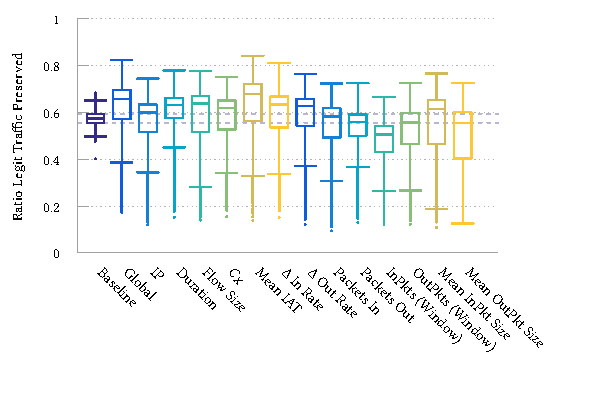
\includegraphics[width=\linewidth]{plots/marl/ftprep-cap-box-thesis}
	\caption[Learnt performance of \emph{Instant} agents when benign traffic is UDP-like, using only a single feature as a basis for decisions.]{
		Learnt performance of \emph{Instant} agents when benign traffic is \gls{acr:udp}-like, using only a single feature as a basis for decisions.
		Mean \gls{acr:iat}, inbound packet sizes, and global state offer the best predictive performance, while most features offer marginal advantage over the unprotected baseline.
		\label{fig:udp-feature-plots}
	}
\end{figure}

\begin{figure}
	\centering
	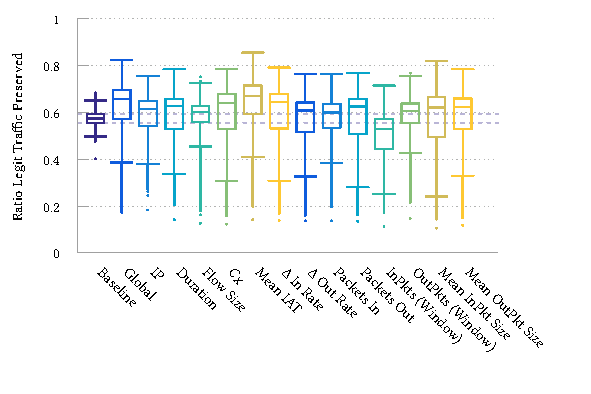
\includegraphics[width=\linewidth]{plots/marl/ftprep-laf-cap-box-thesis}
	\caption[Learnt performance of \emph{Instant} agents when benign traffic is UDP-like, jointly tiling each feature with the last action taken.]{
		Learnt performance of \emph{Instant} agents when benign traffic is \gls{acr:udp}-like, combining each feature with the last action taken as a basis for decisions.
		Compared to \cref{fig:udp-feature-plots}, this combination causes a marked improvement in the packet count and per-window statistics, and leads to a tighter performance bound for Flow Size.
		\label{fig:udp-laf-feature-plots}
	}
\end{figure}

\begin{figure}
	\centering
	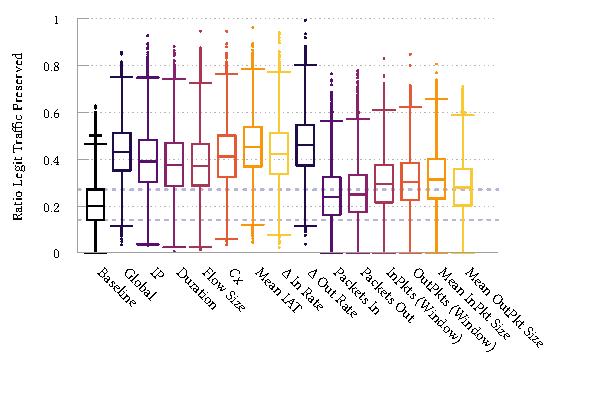
\includegraphics[width=\linewidth]{plots/marl/ftprep-tcp-cap-box-thesis}
	\caption[Learnt performance of \emph{Instant} agents when benign traffic is TCP-like, using only a single feature as a basis for decisions.]{
		Learnt performance of \emph{Instant} agents when benign traffic is \gls{acr:tcp}-like, using only a single feature as a basis for decisions.
		All of the chosen features can offer a marked improvement over no protection at all.
		Global state and Mean \gls{acr:iat} still offer the greatest improvement above baseline, but packet-level statistics are considerably less effective for this class of traffic.
		\label{fig:tcp-cap-feature-plots}
	}
\end{figure}

\begin{figure}
	\centering
%	\vspace{-0.25cm}
	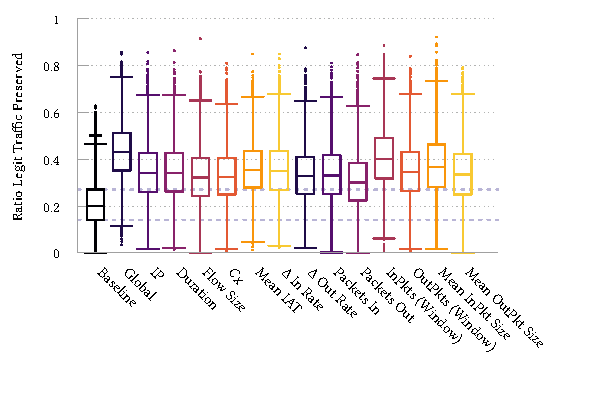
\includegraphics[width=\linewidth]{plots/marl/ftprep-tcp-laf-cap-box-thesis}
	\caption[Learnt performance of \emph{Instant} agents when benign traffic is TCP-like, jointly tiling each feature with the last action taken.]{
		Learnt performance of \emph{Instant} agents when benign traffic is \gls{acr:tcp}-like, combining each feature with the last action taken as a basis for decisions.
		This combination causes a significant improvement in the effectiveness of packet-level and per-window statistics.
		\label{fig:tcp-laf-feature-plots}
	}
\end{figure}

The main element required by a per-source model is a feature set with high predictive power, so that behavioural differences are apparent to an agent.
Elaborating on the statistics discussed in \cref{sec:ddos-motivation} which others have shown to be effective, we believe the following features to be useful (and humanly justifiable), and investigate their use alongside different traffic types.
%?? We use these features, and why...

\paragraph{Global state}
This is the vector of load measurements along a flow's path introduced in \cref{sec:feature-space}.
These values indicate the overall health of the network, and crucially are all measurements which an agent has some degree of direct control over---though the inputs of all agents on all flows are aggregated for later load measurements.

\paragraph{Source IP address}
While trivial to spoof (and thus of limited use for many classes of attack), reflectors are themselves legitimate services being abused by spoofing attackers.
As a result, they communicate with attack victims using their own \gls{acr:ip} address.
In real-world scenarios the addresses of reflector nodes might exhibit similarity due to network uncleanliness~\parencite{DBLP:conf/imc/CollinsSFJWSK07}, e.g., unhardened services exposed by a single organisation.

\paragraph{Last action taken}
This encodes an agent's current belief in the maliciousness of a flow.
This feature also potentially allows forgiveness, serving as a reference point for determining whether a source mistakenly marked as malicious exhibits different falloff behaviour after punishment.
It's important to note that this feature only makes sense once combined with another flow feature, and never appears individually tile-coded.

\paragraph{Flow duration and size}
Features which describe the length of time a connection has been active, and the amount of data transferred within that time.
An extraordinarily long flow, having sent a lot of data, could be more likely to be an amplifier: though most (\qty{62}{\percent}) waves of amplifier traffic last shorter than \qty{15}{\minute}~\parencite{DBLP:conf/raid/KramerKMNKYR15}, this is considerably longer than the typical length of an \gls{acr:http} request/response.

\paragraph{Correspondence ratio}
The ratio between upstream and downstream traffic associated with a source \gls{acr:ip} address.
I define this here as:
$$C_X = \min(\uload{\cdot}, \dload{\cdot})/\max(\uload{\cdot}, \dload{\cdot}),$$
where a value close to 0 indicates strong asymmetry.

\paragraph{$\symbfit{\Delta}$ Send/receive rate}
The change in traffic rates caused by the last action.
Behavioural changes induced by bandwidth expansion or reduction are expected to be most visible here.

\paragraph{Mean inter-arrival time}
A measure of how often packets arrive at an agent's parent switch; low \glspl{acr:iat} indicate a high number of packets per second, and can be a possible marker of malicious behaviour.
I only make use of the mean \gls{acr:iat} of \emph{inbound} traffic.

\paragraph{(Per-window) packet count}
The amount of packets sent to/from a source over a flow's lifetime (or the current window of measurement), similar in use to flow size and mean \gls{acr:iat}.

\paragraph{Mean packet size per window}
Legitimate flows, both congestion-aware and -unaware, often transmit packets with a distribution of sizes.
Attack traffic is not likely to be so diverse: we might expect solely max-size packets in the case of amplification attacks, or minimum-size packets in other flooding attacks.

The exclusion of features such as source/destination ports or protocol numbers is a deliberate choice.
If QUIC or a similar protocol were to become ubiquitous, then these fields would have little to no correlation with the class of traffic a flow might contain.
My aim was to design around this constraint as a form of future-proofing.

\begin{table}
	\centering
	\caption{Tile coding windows for each feature.\label{tab:codings}}
	
%	\resizebox{0.45\linewidth}{!}{
	\begin{tabular}{@{}ll@{}}
		\toprule
		New Feature (unit) & Range \\
		\midrule
		Load (\unit{\mega\bit\per\second}) & $[0, U_s]$ \\
		IP & $[0, 2^{32}-1]$ \\
		Last Action (\unit{\percent}) & $[0, 1]$ \\
		Duration (\unit{\milli\second}) & $[0, \num{2000}]$ \\
		Size (\unit{\mebi\byte}) & $[0,10]$ \\
		Correspondence Ratio & $[0,1]$ \\
		Mean IAT (\unit{\milli\second}) & $[0, \num{10000}]$ \\
		$\Delta$In/Out Rate (\unit{\mega\bit\per\second}) & $[-50, 50]$ \\
		Packets In/Out & $[0, 7000]$ \\
		Packets In/Out Window & $[0, 2000]$ \\
		Mean In/Out Packet Size (\unit{\byte}) & $[0, 1560]$ \\
		\bottomrule
	\end{tabular}
%	}
\end{table}

All of the above features, save for global state, are 1-dimensional.
For simplicity, here `\gls{acr:udp}' refers to congestion-unaware traffic, while `\gls{acr:tcp}' refers to congestion-aware flows.
\Cref{fig:udp-feature-plots} shows the effectiveness of each feature for \gls{acr:udp} (resp.\ \cref{fig:tcp-cap-feature-plots} for \gls{acr:tcp}), on a single-destination topology (\cref{sec:single-dest}) with $n=2$ hosts per egress point averaged over \num{10} runs.
\Cref{fig:tcp-laf-feature-plots} demonstrates how feature accuracy varies when tiled alongside \emph{last action}, with similar trends observed when applied to \gls{acr:udp} traffic (\cref{fig:udp-laf-feature-plots}).
%?? Core findings---different protocols need different features, so everything we proposed above has a use!
The plots show that different protocols and traffic classes are best defended by different features---as such, every feature presented has value in a complete model.
All features converge to their highest-observed performance within around \num{4000} timesteps.
In general, some of the most effective features are the global state, mean \gls{acr:iat}, mean inbound packet size and $\Delta$ rates.
%?? How do they do when combined after individual training? Pretty well, especially for TCP.
%Additional testing shows that the learned per-feature policies may be easily combined (by summing action values), and that this technique is particularly effective for TCP; these results are omitted to preserve space.
%In no cases, however, do we manage to completely block attack traffic---at convergence, we observe that system load remains consistently at $U_s$.

\section{Traffic Modelling}\label{sec:a-new-normal}

%In establishing...
%
%?? How will I structure this?
%?? Motivation -> Model -> Results?
%?? OR Use the results of the last section to springboard into here?

%From what we have seen, it is difficult (or impossible) for trace-based or numerical simulations to correctly capture certain dynamics without an extraordinary amount of care or consideration.
%As it turns out, 
%Our goal is to briefly describe an environment which tests \emph{specific} behaviours to examine the \emph{specific} problems which have arisen during our testing of past approaches.
We contribute network models built around live testing of reactive TCP and UDP traffic in an SDN-enabled environment, which is adaptable to arbitrary topologies, with an explicit focus on preserving their real-time dynamics in a way that trace-based evaluation cannot.
First and foremost, we are interested in representative load and packet inter-arrival characteristics and in how these characteristics evolve in response to actions.
We introduce these models because we are interested in capturing interactive, correlated back-and-forth exchanges associated with live HTTP traffic; mainly because of the particular interactions between the application-level dynamics, congestion awareness at the transport level and the nature of control signal used.
%Naturally, this model is not perfect or representative for all traffic, yet it captures some of the behaviour which we expect will plague most legitimate TCP flows.
%If need be, we expect the frequency or distribution of requests could be conditioned to match observations of real-world access patterns.

%?? ANGLE: set up an environment to test \emph{specific} behaviours to examine \emph{specific} problems in past work. I make no claims that it is perfect or representative for all traffic, just for this (likely common) behaviour which I expect to plague almost all legit TCP flows.

%?? Existing sims used for testing such applications reliant on traces, or not sophisticated enough to capture interactive, back-and-forth (correlated) behaviours---possibly discarded as second-hand effects by past work when these are so crucial given user traffic patterns (and the nature of the control signal we choose to enact).

%?? Remember, the motivation is clear. We don't care so much that it is "representative" wrt a specific deployment location or network type. The whole purpose of this is that we aim to test specific behaviour which traces cannot replicate (i.e., correlated back-and-forth, dynamics introduced to congestion-aware protocols, ...)
%?? If we need to, we can condition the distribution of requests according to statistics mined from an existing trace if reviewer number 2 needs that extra push to be convinced.

\subsection{Network Design}
We make use of a fully software-defined network, built using OpenFlow-aware switches in mininet alongside a controller based on \emph{Ryu} \cite{ryu}.
All internal routers are primed with knowledge of the shortest path to each internal host, while new inbound flows register the ``way back'' for each hop used, to ensure consistent traffic conditions for each flow.
If several ports offer different (equal-length) paths to a destination, a consistent random port is chosen from the flow-hash by an OpenFlow \emph{Group action} (in \emph{select} mode).
If such information is lost, perhaps expiring due to inactivity, it suffices to forward an outbound packet on a random outbound port, as we assume that any external IP is reachable through any of the test network's egress ports (i.e., that it is not connected to any stub ASes).
The controller is also responsible for computing how switches respond to ARP requests: this need arises due to the reliance upon Linux's networking stack for live applications, and wouldn't need to be considered for trace-based evaluation.
%We make further use of the topology presented earlier (\cref{sec:topology}), noting that our architecture allows us to trivially extend and modify this if required.

\subsection{TCP (HTTP) Traffic Model}\label{sec:tcp-http-traffic-model}
%?? Legitimate traffic: TCP traffic (HTTP clients downloading web pages, dependent resources and files) with a mixture of lifetimes for each request.
To model legitimate TCP traffic, server nodes run an nginx v1.10.3 HTTP daemon, serving statically generated web pages alongside various large files and binaries.
Benign hosts run a simple libcurl-based application written in Rust, repeatedly requesting resources from the server.
Hosts and clients both use TCP Cubic \cite{rfc8312}.
Each host's download rate is limited to match the maximum bandwidth assigned to it, and requests several random files known to exist within a website, followed by any dependent resources for each (stylesheets, images, etc.) as a browser might.
On completion, a host changes its IP to generate separate statistics per-flow, while minimising downtime.
This presents a balanced distribution of flow duration and size, with large files included to model elephant flows.

\subsection{UDP (Opus/VoIP) Traffic Model}\label{sec:udp-opus-traffic-model}
VoIP traffic exhibits very different characteristics to the above model; packet arrivals are highly periodic due to real-time requirements, flows have a constant bitrate, and do not react substantially to lost packets.
Interestingly, DDoS attack traffic is known to share many of these characteristics, offering an interesting detection problem.
We present a VoIP traffic model\footnote{\url{https://github.com/FelixMcFelix/opus-voip-traffic}} based on Discord\footnote{\url{https://discord.gg}}, a freely-available messaging and VoIP platform geared toward gaming communities.
We chose Discord as our prototype due to its publicly documented API, many open source bot frameworks, large user base, and due to the lack of models for Opus-encoded traffic.
%?? Highly periodic, CBR

Hosts send RTP traffic with Salsa20 encrypted payloads---\SI{20}{\milli\second} audio frames at \SI{96}{\kilo\bit\per\second}.
We generate similar traffic at hosts by replaying anonymised traces gathered in general use and tabletop RPG servers; each trace contains only the size of each audio payload, entries denoting missed packets, and the duration of silent periods.
We trim these silent periods to a maximum \SI{5}{\second} due to the lengthy talk/silence bursts introduced by users in RPG servers, and estimate the size of missed packets by taking an exponentially-weighted moving average over known sizes.
Hosts punctuate audio frames with a 4-byte keepalive every \SI{5}{\second}.
All traffic passes over a central server which groups hosts into rooms, and is forwarded to other participants; we do not replicate pre-call Websocket traffic which would be used for authentication.
There is no peer-to-peer traffic---the server acts as a TURN relay for all hosts.
%?? Reflective factor among \emph{authenticated hosts}.
We find that each flow occupies an expected \SI{52.4}{\kilo\bit\per\second} upstream bandwidth.
To match the target upload rate assigned to each host, it runs enough individual sessions to meet the target data rate.

%?? Malicious traffic: UDP flood traffic (hping3, MTU-size packets, ). Why not min-size packets? Because the traffic generator gets in a horrible rut if I do so...
\subsection{Attack Traffic Model}\label{sec:attack-traffic-model}
Malicious traffic is generated by use of the \emph{hping3} program, generating UDP-flood traffic targeting random ports.
We configure each instance of \emph{hping3} to generate ethernet MTU-sized packets (\SI{1500}{\byte}) with a random source and destination port towards a target server, and configure the output rate $r$ (in \si{\mega\bit\per\second}) by setting the inter-arrival time $t_{\mathit{attack}}=\frac{1500 \cdot 8}{r\cdot10^6}$.
This fulfils certain characteristics of many types of amplification DDoS traffic: it is congestion-unaware \cite{DBLP:conf/ndss/Rossow14}, and packets are larger than the minimum frame size and identically-sized (e.g., NTP amplification traffic is fragmented at the application layer into \SI{482}{\byte} chunks \cite{cisco-ntp-amp}).
We differ from NTP amplification in frame size so that inter-arrival times are larger, to keep emulation of the network feasible at high traffic rates.

\section{Evaluation}\label{sec:evaluation}
%Traffic is played back from hosts via Tcpreplay at a bandwidth assigned uniformly from a `good' or `bad' distribution, each using the same pcap file with source and destination IP addresses rewritten.

This work is most naturally compared against Marl, introduced by \textcite{DBLP:journals/eaai/MalialisK15}, the state-of-the-art in \gls{acr:rl}-based \gls{acr:ddos} prevention.
We are most interested in seeing how their approach contrasts with the new agent designs across different topologies and workloads.
Different network environments will also impose different levels of host density, where popular web servers may have orders of magnitude more clients than egress points from their network---I aim to show how these characteristics affect performance and learning rate.
Marl is known to outperform the AIMD~\parencite{DBLP:journals/ton/YauLLY05} strategy, yet the state of the art has long since moved on.
To paint a more current picture, I compare this work against an effective modern approach, \emph{SPIFFY}~\parencite{DBLP:conf/ndss/KangGS16}.
SPIFFY tests a proportion of flows by routing them through an alternate path with higher bandwidth, observing how their speed changes some time later.
This comparison lets us position our new agent designs against the state of the art, observing that SPIFFY has a similar mode of interaction to \gls{acr:rl}-based systems (taking action, observing an effect, and acting once again) and does not rely on protocol characteristics or signatures.
In reimplementing SPIFFY, I make the simplifying assumption that a suitable unused path exists (with identical bandwidth to the server's link).
\qty{10}{\percent} of active flows were tested at a time (according to the authors' observation that there is a factor of \qty{10}{\times} difference between the ideal and achieved bandwidth expansion), excluding flows below \qty{50}{\kilo\bit\per\second} and requiring a \qty{3}{\times} expansion from legitimate flows, making a judgement after \qty{5}{\second}.

To test this, I made use of both traffic models introduced in \cref{sec:a-new-normal} (Opus and \gls{acr:tcp}), both topologies discussed below (1-dest vs.\ Fat-Tree), and vary the amount of hosts typically communicating over each agent's ingress/egress node.
Additionally, these new models were evaluated in multi-agent mode (\emph{separate}, no model sharing), and in single-agent mode (\emph{single}, zero-cost perfect information sharing).
In each case, the algorithm's performance was averaged over \num{10} episodes of length \num{10000} timesteps (setting each agent's $\wvec{}=\mathbf{0}$ between episodes).
Host allocations at the beginning of each episode were generated pseudorandomly to ensure fairness between episodes---a host is malicious with probability $\operatorname{P}\left(\mathit{malicious}\right)$, and is benign otherwise.
Benign hosts generate traffic according to either \cref{sec:tcp-http-traffic-model,sec:udp-opus-traffic-model} depending on the experiment, while malicious hosts generate traffic as described in \cref{sec:attack-traffic-model} (both at experiment-dependent rates).

All experiments were executed on Ubuntu 18.04.2 LTS (GNU/Linux 4.4.3-040403-generic x86\_64), using an Intel Core i7-6700K (\qtyproduct[product-units=single]{4 x 4.2}{\giga\hertz}) which had \SI{32}{\gibi\byte} of \gls{acr:ram}.
%All code underpinning these findings is available on a public repository\footnote{\url{https://github.com/FelixMcFelix/rln-dc-ddos-paper}}.
%All code underpinning these findings is available on a public repository.\footnote{Private until publication.}

\subsection{Single destination}\label{sec:single-dest}
%?? Move description of tree topol to here.
The network is tree-structured, where one server $s$ connects through a dedicated switch to $k$ team leader switches, each connected to $\ell$ intermediate switches, which in turn each connect to $m$ egress switches.
We then have $N_{\mathit{hosts}} = k \ell m n$.
\Cref{fig:marl-topol} demonstrates this.
%Although \citeauthor{DBLP:journals/ccr/MahajanBFIPS02a}, the originators of this topology, make it clear that it exists as a fairly unrepresentative example \cite{DBLP:journals/ccr/MahajanBFIPS02a}, it remains the case that such a network topology allows for functional testing, and indeed is illustrative of one way in which attack traffic might aggregate in the network.
%It is hard, however, to argue its relevance to specific classes of victim or to reason about the interactions it might have with dependent applications.
%We aim to address this through \cref{sec:performance-in-an-emulated-environment}.
The network topology was configured using $k=2$ teams, $\ell=3$ intermediate nodes per team, $m=2$ agents per intermediate node, and $n \in \{2, 4, 8, 16\}$ hosts per learner.
This is a slight simplification of \Textcite{DBLP:journals/eaai/MalialisK15}'s \textquote{online} experiment, choosing fewer teams but remaining as a single server with a fan-out network.
%The algorithm parameters were set at $\gamma=0$ (leading to opportunistic behaviour), $\alpha=0.05$, having linearly annealed $\epsilon=0.2 \rightarrow 0$ by $t=3000$.
%Benign and malicious hosts uploaded between \SIrange{0}{1}{\mega\bit\per\second} and \SIrange{2.5}{6}{\mega\bit\per\second} respectively, and hosts were redrawn at each episode's start with $\operatorname{P}(\mathit{malicious})=0.4$.
%$U_s$  $k \ell mn+2$ \si{\mega\bit\per\second}.
%The performance of each choice of $n$ was averaged over \num{10} episodes of length \num{10000} timesteps (setting each agent's $\wvec{}=\bm{0}$ between episodes).
%Host allocations were generated pseudorandomly to ensure fairness between choices of $n$.
%These parameter choices match those of the original study to enable direct comparison, and are (to the best of our knowledge) arbitrary, but we justify our range of $n$ as capturing increasing scales of host activity.

\begin{figure}
	\centering
	\resizebox{0.9\linewidth}{!}{\begin{tikzpicture}[
	texts/.style = {text=black},
	labeltexts/.style = {text=uofgsandstone},
	treeline/.style = {draw=uofgburgundy},
	treenode/.style = {texts, circle, centered, fill=white, treeline},
	load/.style = {fill=uofgcobalt},
	loadhide/.style = {fill=uofgcobalt!40!white},
	external/.style = {fill=uofgrust},
	externalhide/.style = {fill=uofgrust!40!white},
	hideline/.style = {draw=uofgsandstone!40!white},
	hidenode/.style = {treenode, hideline},
	grow'=right
]
	\node[treenode, label={[texts]above:Server}] (root) {}
	child [treeline] { node [treenode, label={[texts]above:Core}] (sswitch) {}
		child [treeline] { node [treenode, label={[texts]above:Leader}] (teaml) {} 
			child [treeline] { node [treenode, label={[texts]above:Intermediate}] (inter) {}
				child [treeline] { node [treenode, load, label={[texts]above:Agent/Egress}] (agent) {}
					child [treeline] { node [treenode, external] (extern) {}
						child [treeline] { node [treenode, external, label={[texts]above:Host}] (host) {} }
						child [hideline] { node [hidenode, externalhide] (endhost) {} }
					}
				}
				child [hideline] { node [hidenode, loadhide] (endagent) {} }
			}
			child [hideline] { node [hidenode] (endinter) {} }
		}
		child [hideline] { node [hidenode] (endteaml) {} }
		edge from parent
		node[below, labeltexts] {$U_s$}
	};
	
	%\draw[-] (teaml) -- (endteaml);
	\node [labeltexts] (kdots) at ($(teaml)!0.5!(endteaml)$) {$\rvdots$};
	\node [labeltexts, right = -0.1cm of kdots] {$k$};
	\node [labeltexts] (ldots) at ($(inter)!0.5!(endinter)$) {$\rvdots$};
	\node [labeltexts, right = -0.1cm of ldots] {$\ell$};
	\node [labeltexts] (mdots) at ($(agent)!0.5!(endagent)$) {$\rvdots$};
	\node [labeltexts, right = -0.1cm of mdots] {$m$};
	\node [labeltexts] (ndots) at ($(host)!0.5!(endhost)$) {$\rvdots$};
	\node [labeltexts, right = -0.1cm of ndots] {$n$};
\end{tikzpicture}}
	\caption[Tree-structured network topology diagram for evaluating a single-destination network.]{
		Network topology diagram, showing how the server and its core switch's $k$ teams are structured, with $\ell$ intermediate routers per team, connected to $m$ agents which each moderate $n$ hosts beyond a single external switch.
		%	Empty nodes are considered to be internal.
		Red nodes are external, and each blue node hosts an agent.
		\label{fig:marl-topol}
	}
\end{figure}

\subsection{Multiple destinations}
The previous topology allows for direct comparison against the state-of-the-art, and indeed is illustrative of one way in which attack traffic might aggregate in the network.
It is hard, however, to argue its relevance to specific classes of victim or to reason about the interactions it might have with dependent applications.
In contrast, the fat-tree topology~\parencite{DBLP:conf/sigcomm/Al-FaresLV08} sees regular use in real-world data centres and scales well horizontally.
%?? Come up with description of fat-tree (multi-dest) topol.
%?? Why fat tree? regularly appears in modern datacentres.
%?? $k=4$ fat-tree , with one pod hosting two servers $s_0,s_1$.
We use a $k=4$ fat-tree, with one pod hosting two servers $s_0$ and $s_1$.
$n$ external hosts connect through each core switch (where agents are hosted), and communicate with $s_0, s_1$ uniformly randomly.
Both servers host identical services.
We set $n \in \{6, 12, 24, 48\}$ hosts per learner (keeping $N_{\mathit{hosts}}$ identical to each tier of the single-host topology), and restrict $U_{s_0} = U_{s_1} = U_s / 2$.

\subsection{Parameters}
The algorithm parameters were set at $\alpha=$~\num{0.05}, linearly annealing $\epsilon=$ \num{0.2} $\rightarrow$ 0 by $t=$~\num{3000} in the case of Marl (\num{8000} actions per agent in the \emph{Instant/Guarded} models).

Benign hosts each occupied \qtyrange{0}{1}{\mega\bit\per\second}, and hosts were redrawn at each episode's start with $\operatorname{P}(\mathit{malicious})=$~\num{0.4}.
%The original introduction of this approach to direct-control reinforcement learning as introduced by \textcite{DBLP:journals/eaai/MalialisK15} fails to consider key cases: the absence of a suitable heuristic classifier $g(\cdot)$, disjoint ranges of traffic distribution (i.e., the presence of benign heavy-hitters), the accurate simulation of TCP-like behaviour (and its effects on collateral damage), and high densities of hosts at egress points.
%?? Why? ...
%Of these, the latter two are most deserving of a closer investigation, as they have stronger implications for wide-scale deployment.
%These are important issues, particularly when we consider real-world deployment.
%Heuristic estimates of traffic legitimacy come with computational cost and couple the reward function to the accuracy of the estimator, hosts often show diversity in their own traffic patterns (perhaps being multi-modal), and it is known that TCP is the most used transport protocol for Internet traffic \cite{DBLP:conf/saint/ZhangDJC09}.
%?? NEED TO VERIFY VOLUME OF CONGESTION-AWARE PROTOCOLS
Malicious hosts each sent \qtyrange{2.5}{6}{\mega\bit\per\second} when attacking \gls{acr:udp} traffic, though this was increased to \qtyrange{4}{7}{\mega\bit\per\second} when using \gls{acr:tcp}-like traffic (to meaningfully impact benign flows).
Given $n$ and $\operatorname{P}(\mathit{malicious})$, we see an expected malicious bandwidth \numrange{1.27}{1.87} and \qtyrange{2.03}{2.18}{\times} $U_s$ respectively.
%The expected fraction of $U_s$ consumed by each host is \SI{21.5}{\percent} for $n=2$, and \SI{2.84}{\percent} for $n=16$.
For these choices of $n$ in both topologies, we observe $N_{\mathit{hosts}} \in \left\{24, 48, 96, 192\right\}$, and an expected number of malicious hosts $\mathbb{E}\left[N_{\mathit{attackers}}\right] \in \left\{9.6, 19.2, 38.4, 76.8\right\}$.
For the largest choice of $n$, we see an expected total attack traffic $\mathbb{E}\left[V_{\mathit{attack}}\right] =$ \qtylist{334.05;422.4}{\mega\bit\per\second} for Opus and \gls{acr:http} traffic respectively.

$U_s$ was fixed at $N_{\mathit{hosts}}+2$ \unit{\mega\bit\per\second} (to account for burstiness), and each link had a delay of \qty{10}{\milli\second}.
All links had unbounded capacity, save for each server-switch.
These parameters match those of the original study to enable direct comparison, and many are (to the best of our knowledge) arbitrary, but I justify the range of $n$ as capturing increasing scales of host activity.

\section{Results}\label{sec:the-results-of-doing-so}
?? Exec summary in top-of-line?

\subsection{Raw inference and learning performance}
\Cref{tab:lats} shows how \approachshort{} compares in latency with a numpy-based RL policy.\footnote{For brevity, we omit numpy-based integer results---against a floating point implementation, median action latencies are \qty{14.6}{\percent} worse, with \qty{7.9}{\percent} longer update times.}
We show that \Coopfw{} achieves sub-\qty{35}{\micro\second} median latency, with \nth{99} and \num{99.99}\nthscript{th} percentile latencies less than \qty{1}{\micro\second} worse using 4 MEs of the NFP-6480.
This corresponds to \qtylist{15;21}{\times} speedups over a \emph{Collector} host.
Importantly, \Indfw{} achieves lower median state-action latencies (\qty{2.79}{\times}) \emph{and} update times (\qty{2.63}{\times}) than a dedicated \emph{Collector} host \emph{while requiring only a single core or dedicated functional unit}.

\newlength{\resultplotwidth}
\setlength{\resultplotwidth}{\linewidth}

\begin{table}
	\caption{Latencies and computation times for \approachshort{} versus commodity hardware hosts. On-device execution is crucial in not only lowering latencies, but in reducing tail latencies. Lower is better, with the best marked \emph{in bold}.\label{tab:lats}}
	\resizebox{\linewidth}{!}{
		\expandableinput tables/opal/latency-only32
	}
\end{table}

\begin{table}
	\caption{Action and update throughputs for \approachshort{} versus commodity hardware hosts. Most designs cannot scale online performance with additional cores. Higher is better, with the best marked \emph{in bold}.\label{tab:tputs}}
	\resizebox{\linewidth}{!}{
		\expandableinput tables/opal/tput-only32
	}
\end{table}

\Cref{tab:tputs} compares \approachshort{}'s throughput against host-based execution.
We set the worker count on host machines which maximised their throughput.
This equalled the amount of physical cores on each device---moving beyond this (even below the number of hyper-threads) would hamper tail latencies by an order of magnitude.
To make the comparison fair in the context of many-core CPU environments, we include per-core throughput.
\Indfw{} achieves \qty{2.82}{\times} higher offline throughput than commodity \emph{Collector} hardware in spite of the NFP-6480 having a considerably slower clock speed (\qty{0.29}{\times}).
When compounded with the abundance of such weaker chips, in-NIC RL is able to deliver much higher throughput.
%As anticipated, the \Coopfw{} strategy is key in achieving serviceable throughput in an online learning agent, \qty{9.9}{\times} that of a dedicated collector machine, due to the locking requirements mandating coordinated division of work.
As anticipated, the \Coopfw{} strategy is key in achieving serviceable throughput in an online learning agent, \qty{9.9}{\times} that of a dedicated collector machine, as the write lock around policy updates creates a bottleneck.

By limiting the available workers in software, we show how \Coopfw{}'s policy update time (thus  online throughput---\cref{fig:vary-core}) and state-action latency (\cref{fig:vary-core-latency}) scale with available cores.
While \Coopfw{} always outperforms the host-based floating point implementations, we observe that there are two distinct crossover points which must be met to overcome our own \Indfw{}; \num{8} workers for online throughput, and \num{3} workers for state-action latency.
Some artefacts of our environment and design choices are visible, such as the addition of new physical cores being more significant than contexts, and the presence of some schedule bottlenecks.
Most importantly however, \Coopfw{}'s resource demand is tunable at compile time to meet the online training rate and/or action latency required by a task/environment.

\begin{figure}[t]
	\resizebox{\resultplotwidth}{!}{
		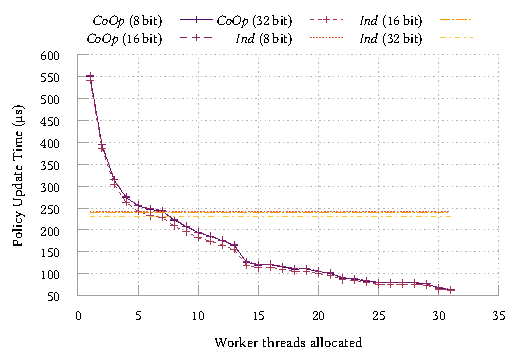
\includegraphics{plots/opal/rl-perf-tester/vary-core}
	}
	\caption{
		\Coopfw{}'s online learning performance improves with additional cores, on max size tasks (\num{129} work items). This requires \num{8} workers to offer greater online throughput than single-threaded in-NIC RL. Sharper performance increases occur when a new physical core is added (\numrange{7}{8}) or the scheduler works around a bottleneck (\numrange{13}{14}).\label{fig:vary-core}}
\end{figure}

\begin{figure}
	\resizebox{\resultplotwidth}{!}{
		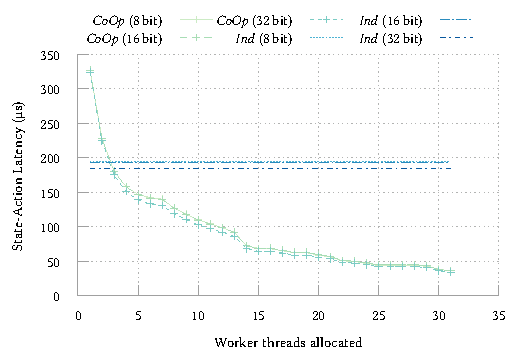
\includegraphics{plots/opal/rl-perf-tester/vary-core-latency}
	}
	\caption{\Coopfw{}'s action latencies similarly improve with more cores. This requires \num{3} workers (4 total contexts) to improve upon the state-action latency of single-threaded in-NIC RL.\label{fig:vary-core-latency}}
\end{figure}

\Cref{fig:vary-work,fig:vary-work-latency} show how policy complexity affects update cost and state-action latency respectively, scaling from a bias tile up to the full DDoS policy size.\footnote{Input vectors here all have 20 elements regardless of the policy design.}
\Coopfw{} always produces an action in less time than \Indfw{}, but requires at least one state-based tile to excel in online learning.
%We note that this is a trivial case, in that the use of \emph{only} a bias tile negates the need for any input state (similar to a multi-arm bandit problem).
We note that this is a trivial case, as using \emph{only} a bias tile returns a single preference list regardless of input state.

We found that a key aspect of in-NIC execution is that it allows far tighter bounds on tail latency compared to host offloading.
Examining the state-action latencies in \cref{tab:lats}, we see that \num{99.99}\nthscript{th} percentile latencies exceed the median by \qtylist{0.58;0.66}{\percent} for \Indfw{} and \Coopfw{}, respectively.
Similar results were observed for other bit depths.
By contrast, host-based tail latencies are at least \qty{40.53}{\percent} greater even when the parallel worker count is at or below the physical core count.
We show the cumulative distributions of these in detail (\cref{fig:lat-cumul}), noting how just one additional CPU-intensive task---potentially automated system updates, scans, or another vNF/traffic processing task---impacts tail latencies further (\emph{Float(Over)}).

\begin{figure}[t]
	\resizebox{\resultplotwidth}{!}{
		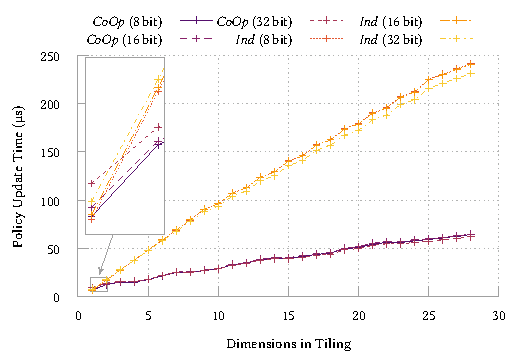
\includegraphics{plots/opal/rl-perf-tester/vary-work}
	}
	\caption{\Coopfw{} fully processes updates faster than \Indfw{}---thus has higher online performance---on almost all policy sizes. Lower bit depths are more effective on simpler policies.\label{fig:vary-work}}
\end{figure}

\begin{figure}
	\resizebox{\resultplotwidth}{!}{
		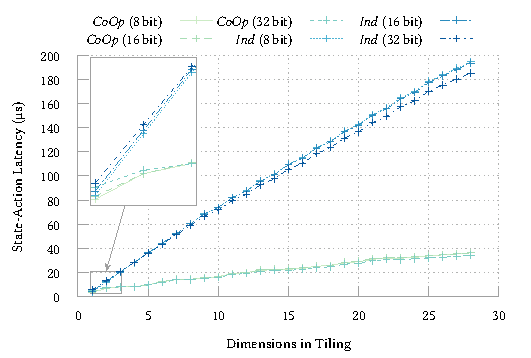
\includegraphics{plots/opal/rl-perf-tester/vary-work-latency}
	}
	\caption{State-action latency scales with additional work in a similar manner to overall processing time; though \qty{32}{\bit} firmwares become more effective sooner (at \num{3} work items).\label{fig:vary-work-latency}}
\end{figure}

\begin{figure}
	\centering
	\begin{subfigure}{\linewidth}
		\resizebox{1.0\linewidth}{!}{
			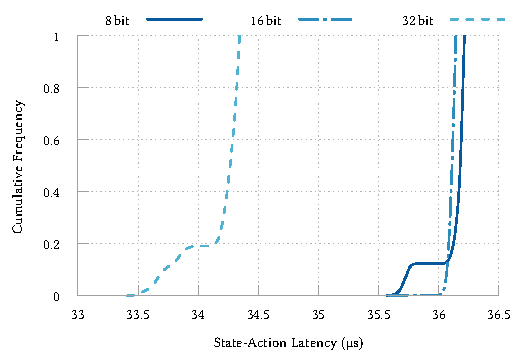
\includegraphics{plots/opal/rl-perf-tester/latency-cumul-thesis}
		}
		\caption{\approachshort's \Coopfw{} design achieves consistent, tight latency bounds.}
	\end{subfigure}

	\begin{subfigure}{\linewidth}
		\resizebox{1.0\linewidth}{!}{
			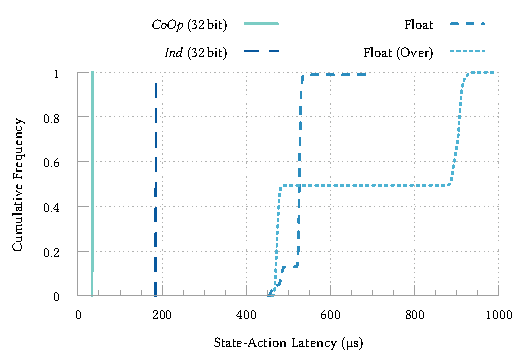
\includegraphics{plots/opal/rl-perf-tester/latency-cumul-broad-thesis}
		}
		\caption{Tail latencies suffer in hosts---particularly when oversubscribed.}
	\end{subfigure}
	\caption{Cumulative state-action latency plots for \approachshort{} and host-based execution.\label{fig:lat-cumul}}
\end{figure}

A noteworthy trend is that \qtylist{8;16}{\bit} versions of \approachshort{} consistently underperform compared to \qty{32}{\bit}, except for smaller workloads (seen in the zoomed portions of \cref{fig:vary-work,fig:vary-work-latency}).
This occurs even though our implementation is optimised to read and write policy data in batches (achieving fewer I/O operations).
We see this because the native register width on the NFP is \qty{32}{\bit}, and so the compiler must emit extra instructions around arithmetic operations to correctly load and update values.
This matches \qty{32}{\bit} becoming dominant in complex workloads: higher dimension tilings require more arithmetic operations.
Most of the I/O comes \emph{after} this step, causing ALU use to dominate.
This also explains why \qty{32}{\bit} becomes the best choice at different policy complexities for online (\cref{fig:vary-work}, 10 dims) and offline (\cref{fig:vary-work-latency}, 3 dims) agents, where hashtable accesses and a \texttt{memcpy} of the state vector fall into the serial portion of the online algorithm.
Smaller bit depths still give a \qtyrange{2}{4}{\times} saving in memory for policy storage (enabling more fine-grained or complex policies), in exchange for slightly worse latency and throughput.
To overcome this, we investigated bit-stuffing several values into a single word during atomic writeback (as the platform offers both \qtylist{32;64
}{\bit} atomic addition).
This is analogous to SIMD through clever use of padding bits, but we found that manipulating tiles into the correct format added \qty{10}{\percent} extra overhead.

\subsection{Work allocation}
\Cref{fig:work-alloc-32} shows that our heuristic allocator (\emph{Balanced}) is key in achieving consistent sub-\qtylist{35;65}{\micro\second} latencies/update times, respectively.
The trend is repeated for all bit depths.
The constant difference between \emph{Action} and \emph{Update Prep} scales linearly with bit depth, matching storage and lookup work in the serial portion of \emph{ParSa} (plots omitted).
The severe underperformance of the \emph{Na\"{i}ve} allocator confirms that work item complexity is correlated with its index, as batching work in contiguous chunks gives some workers only high-dimensionality tilings.
The minor gap in lower bound performance between the \emph{Random} and \emph{Balanced} allocators suggests that further optimisations can be made.
We expect that closing or exceeding this gap may require more complex modelling of hardware thread interactions, which lies far beyond the scope of in-NIC scheduling.
Some additional complexity may be tolerated, subject to code store limits---scheduling runs exactly once per configuration change, so does not impact per-action code.

\begin{figure}
	\resizebox{\resultplotwidth}{!}{
		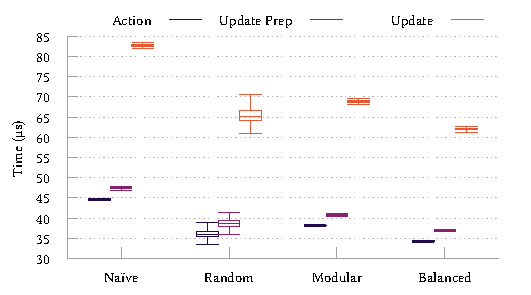
\includegraphics{plots/opal/rl-perf-tester/work-strat-32bit}
	}
	\caption{Action/update compute times in a \qty{32}{\bit} \Coopfw{} agent under different work schedulers.\label{fig:work-alloc-32}}
\end{figure}

\begin{figure}
	\resizebox{\resultplotwidth}{!}{
		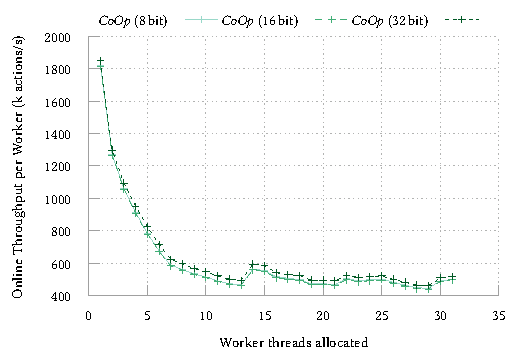
\includegraphics{plots/opal/rl-perf-tester/vary-core-tput-on-per}
	}
	\caption{Throughput per added worker in a \Coopfw{} agent.\label{fig:tput-per-core}}
\end{figure}

An interesting aspect of \Coopfw{} and \emph{ParSa} is that adding cores has both diminishing returns and key thresholds to pass.
Consider \cref{fig:tput-per-core}, where the throughput per worker decreases with cores but occasionally increases sharply.
Later downward ticks (\numrange{25}{29} workers) correspond to plateaus in throughput.
This is a problem stemming from the granularity of work items (i.e., tilings in \emph{ParSa}), where our scheduler cannot find a better solution to a bottleneck until extra cores are allocated.
We measured individual work items in state-action computation to take a mean \qtylist{5.2; 6.2; 9.7; 11.0}{\micro\second} for bias, CLS, CTM and IMEM tilings respectively.
Though we have a \qty{4.2}{\times} factor of task oversubscription, it is clear that latencies are eventually bound below by the length of the longest task.

\subsection{End-to-end RL latency}
%?? PCIe RTT is 10us (neugebauer, BNN NFP paper), NFP RTT is 18us (own measurements). EMEM Ring one-way is 120ns.
%?? Cziva~\parencite[pp.113]{DBLP:phd/ethos/Cziva18} discusses vNF times.
%?? reference the inference times brought up in Taurus?
Referring to \cref{fig:state-slip}, we take $t_2$ from \cref{tab:lats} for host and in-NIC processing times, and substitute $t_1+t_3$ for the state packet round-trip time to the decision site:
\begin{description}
	\item[In-NIC.] As described in \cref{sec:agent-environment-communication}, EMEM rings have a median one way delay cross-island of \qty{140}{\nano\second}, giving a \emph{median \qty{34.63}{\micro\second} end-to-end inference latency}.
	\item[Dedicated Collector.] Offloads hosted in this manner will employ DPDK to maximise performance, giving one-way PCIe delays of \qtyrange{0.9}{2.3}{\micro\second} for network packets~\parencite{DBLP:conf/sigcomm/NeugebauerAZAL018}.
	A UDP packet carrying \num{20} elements of state in \approachshort{} is \qty{128}{\byte}, so costs \qty{1}{\micro\second} to forward, and the reply state-action pair is slightly larger.
	\emph{This gives an end-to-end inference latency of \qty{517.9}{\micro\second}}.
	\item[vNF Offload.] \Textcite{DBLP:journals/cm/CzivaP17} show that more lightweight vNF frameworks like GNF~\parencite{DBLP:journals/cm/CzivaP17} and ClickOS~\parencite{DBLP:conf/nsdi/MartinsAROHBH14} add \qtyrange{45}{55}{\micro\second} \emph{additional} RTT latency above PCIe costs.
	\emph{This gives an end-to-end inference latency of \qty{572.9}{\micro\second}}.
\end{description}
Using these estimates, in-NIC classical RL inference offers \qtylist{14.96;16.54}{\times} speedups in latency over collector and vNF deployments respectively (assuming no steering cost in either case).
We also contrast these against deep RL policies on network tasks, which can take \qty{3}{\milli\second} to compute~\parencite{DBLP:journals/corr/abs-1910-04054}---2 orders of magnitude above \approachshort{} with identically sized (20-dim) input vectors.
%In the name of fairness, we assume that rule installation uses same mechanism we recommend, but show how bad it can get? I.e. with rule installation costs etc.

\subsection{Co-existence with the dataplane}
Our setup met \qty{40}{\giga\bit\per\second} for packet sizes $\ge$\qty{256}{\byte}.
%For frame sizes of \qtylist{64;128;256}{\byte} input traffic rates were \qtylist{17.4;32.9;37.0}{\giga\bit\per\second} respectively (\qtylist[per-symbol=p,sticky-per=true]{33.9;32.2;18.1}{\mega\packet\per\second}).
For frame sizes of \qtylist{64;128}{\byte}, input traffic rates were \qtylist{17.4;32.9}{\giga\bit\per\second} respectively (\qtylist[per-symbol=p,sticky-per=true]{33.9;32.2}{\mega\packet\per\second}).
Passing this traffic over the NFP device running \approachshort, no packet losses were incurred at any rate of RL actions.

We show the effect of RL workloads on the round-trip latencies of cross traffic through \cref{fig:dataplane-coop}.
As observed latencies do not obey a normal distribution (particularly \qtylist{256;1518}{\byte}, which are bimodal), we employ a one-tailed \emph{Mann-Whitney U test} to mark statistically significant population increases in latency ($p < 0.05$) with a ``+''.
In general, statistically significant latency increases concentrate around smaller packet sizes.
All (bar one) of these affected \nth{99} percentile latencies by under \qty{0.38}{\percent} (at most \qty{78}{\nano\second}).
This slight degradation can be explained by increased pressure on the NFP's \emph{Command Push-Pull} (CPP) bus, which is responsible for handling cross-island accesses to memory (particularly IMEM/EMEM) and other resources.
\approachshort{} places load on the CPP bus through its \inring{}/\outring{} EMEM rings and last-tier policy accesses.
This also explains the sensitivity of \qty{256}{\byte} packets to \approachshort{}---the NFP P4 toolchain segments packets, storing metadata (e.g., MAC prepend) and the first bytes of a packet in a \qty{256}{\byte} CTM block and parking their payloads in EMEM.
\qty{256}{\byte} packets overshoot this due to metadata, causing small I/O accesses at a high rate for packets sized around this cutoff.
%Regardless, this effect is small when observed.

The anomalous result is \qty{128}{\byte} packets at \num{3000} RL action/update computations per second, causing a \qty{222}{\nano\second} (\qty{1.18}{\percent}) increase, shown in \cref{fig:dataplane-example}.
This is observed through a shift of some packet latencies from the mode towards the tail, but no other changes in the distribution.
In the above context, we believe that the inbound request rate is weakly synchronised with inbound packets, causing a higher level of burstiness around accesses to the CPP bus.
We expect that dedicated hardware/FPGA designs can avoid this problem by having dedicated \inring{}/\outring{} access mechanisms for an \approachshort{} agent.

\begin{figure}
	\centering
	\begin{subfigure}{0.45\linewidth}
		\resizebox{1.0\linewidth}{!}{
%			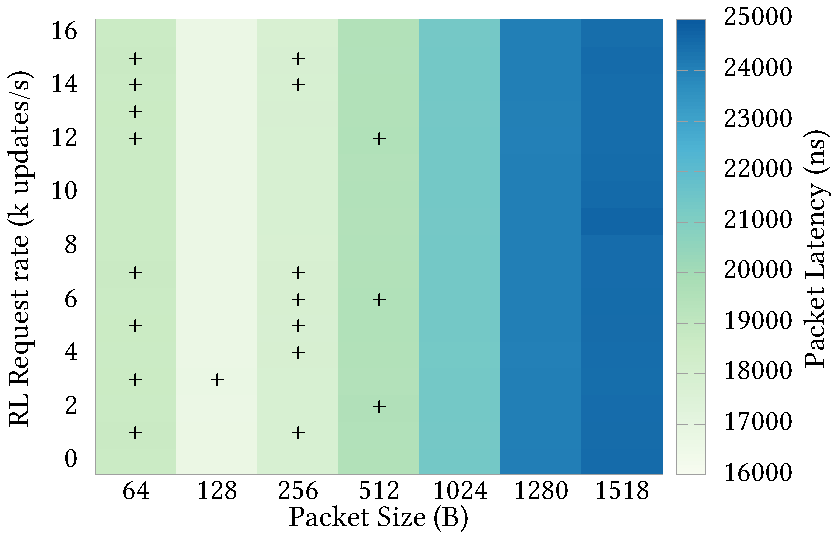
\includegraphics{../plots/build/stress/heat-latency-median}
			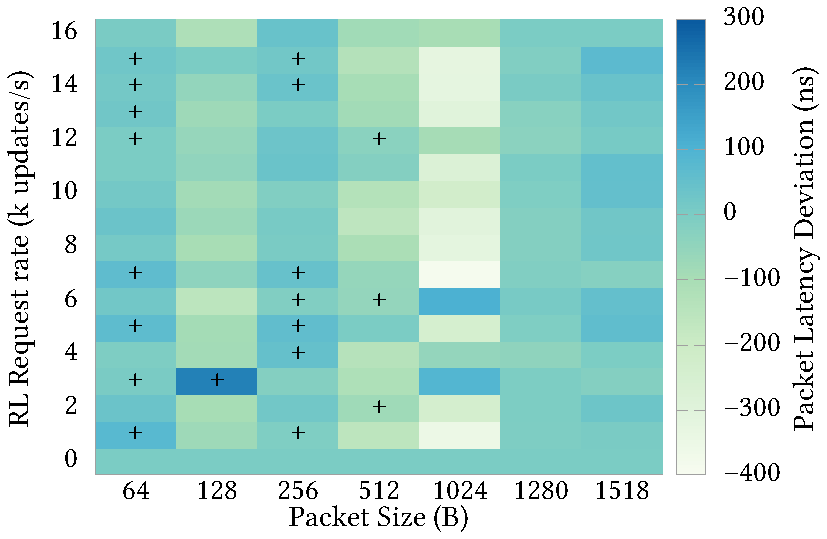
\includegraphics{plots/opal/stress/heat-latency-two-9-rel}
%			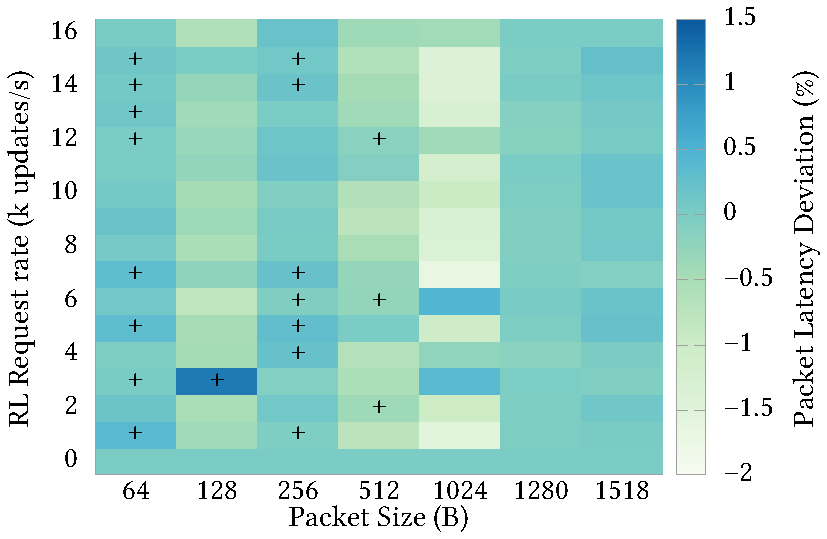
\includegraphics{../plots/build/stress/heat-latency-two-9-perc}
		}
		\caption{Deviations in \nth{99} percentile cross-traffic RTTs.\label{fig:dataplane-heat}}
	\end{subfigure}
	\hspace{0.05\linewidth}
		\begin{subfigure}{0.45\linewidth}
		\resizebox{1.0\linewidth}{!}{
			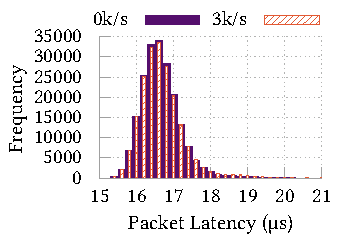
\includegraphics{plots/opal/stress/histo-128B-0-3-trim}
		}
		\caption{Distribution of RTTs for \qty{128}{\byte} packets for \numlist{0;3000} RL actions/s.\label{fig:dataplane-example}}
	\end{subfigure}
	\caption{Effects on tail latency of cross-traffic caused by different loads of off-path RL compute. Statistically significant increases in population latency are concentrated on smaller packet sizes, and are typically sub-\qty{78}{\nano\second}.\label{fig:dataplane-coop}}
\end{figure}

\subsection{Resource requirements}
\Cref{tab:resources} shows how \approachshort{} consumes shared memory as it scales to fit a device's compute resources, compared with a simple P4 forwarding application.
As one program is installed per ME, these results represent the minimum and maximum resource use on a single island (i.e., without replacing P4 workers).
We observe negligible costs on shared EMEM ($\sim$\qty{4}{\mebi\byte}), incurred due to hashtables for past state and rewards.
The most significant costs arise due to policy data (\qty{405}{\kibi\byte} shared IMEM, \qty{90}{\kibi\byte} local CTM, \qty{15}{\kibi\byte} local CLS), which can be halved or quartered using \qtylist{16;8}{\bit} quantisation and remain constant regardless of compute unit usage.
This is a high upfront cost on per-island resources (CLS/CTM)---\approachshort{} leaves resources for other off-path dataplane applications, but is fairest from 3 cores onwards.

%Thread local storage in CLS for compute/register spilling scales with the number of MEs required (requiring \qtylist{13.77;15.49}{\percent} per-ME for \Indfw{}/\Coopfw) due to precaching and the space needed to hold tile lists.
%Due to the initial policy cost this falls below the fair share at 3 MEs, but always allows for co-existence with other asynchronous dataplane programs.

\begin{table}
\caption{NFP memory use due to \approachshort{} using \numlist{1;4} MEs (\qty{32}{\bit}). CLS and CTM are shared between all programs on the same island (placing our RL agent on i5), while EMEM and IMEM are shared between all NFP programs on a NIC.\label{tab:resources}}
\resizebox{\linewidth}{!}{
\begin{tabular}{
		@{}c
		S[table-format=4.2] S[table-format=2.2]
		S[table-format=4.2] S[table-format=2.2]
		S[table-format=4.2] S[table-format=2.2]
		S[table-format=2.2] S[table-format=2.2]
		S[table-format=3.2] S[table-format=2.2]
		@{}
	}
	\toprule Firmware & \multicolumn{2}{c}{EMEM} & \multicolumn{2}{c}{EMEM Cache} & \multicolumn{2}{c}{IMEM} & \multicolumn{2}{c}{i5.CLS} & \multicolumn{2}{c}{i5.CTM}\\
	& \multicolumn{1}{c}{\si{\mebi\byte}} & \multicolumn{1}{c}{\si{\percent}} & \multicolumn{1}{c}{\si{\kibi\byte}} & \multicolumn{1}{c}{\si{\percent}} & \multicolumn{1}{c}{\si{\kibi\byte}} & \multicolumn{1}{c}{\si{\percent}} & \multicolumn{1}{c}{\si{\kibi\byte}} & \multicolumn{1}{c}{\si{\percent}} & \multicolumn{1}{c}{\si{\kibi\byte}} & \multicolumn{1}{c}{\si{\percent}} \\
	\midrule Base P4 & 6776.67 & 88.24 & 268.52 & 2.91 & 858.28 & 10.48 & 0.00 & 0.00 & 0.00 & 0.00 \\
	\Indfw(1) & 6780.21 & 88.28 & 2541.08 & 27.57 & 1263.28 & 15.42 & 24.75 & 38.67 & 94.25 & 36.82 \\
	\Indfw(4) & 6780.22 & 88.28 & 2545.33 & 27.62 & 1263.28 & 15.42 & 51.18 & 79.97 & 107.00 & 41.80 \\
	\Coopfw(1) & 6779.12 & 88.27 & 1773.59 & 19.24 & 1263.28 & 15.42 & 22.41 & 35.01 & 90.00 & 35.16 \\
	\Coopfw(4) & 6779.12 & 88.27 & 1769.84 & 19.20 & 1263.28 & 15.42 & 52.16 & 81.49 & 90.00 & 35.16 \\
	\bottomrule
\end{tabular}
}
\end{table}

%\paragraph{The impact of bit depth}
%?? \Cref{fig:quant-acc}
%?? \qty{5}{\bit} mantissa suffices for $\ge$ \qty{90}{\percent} relative accuracy, so \qty{8}{\bit} is fine (1S + 2E + 5M), \qty{16}{\bit} is better.
%
%\begin{figure}
%	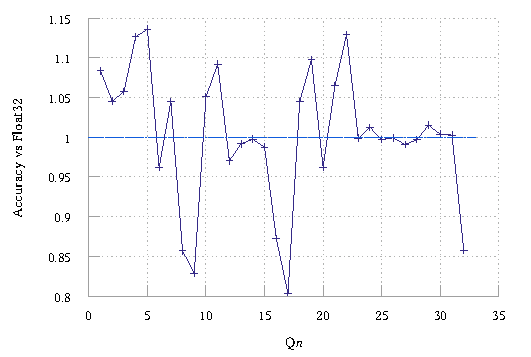
\includegraphics{../plots/build/marl-quant/accuracy-binary}
%	\caption{Normalised accuracy of a converted, pre-trained floating-point tile-coded policy after conversion to $32Qn$ fixed-point.}\label{fig:quant-acc}
%\end{figure}

\subsection{Deployability}
Setup of \approachshort{} uses two packet types: \emph{setup}, which contains learning (hyper-)parameters and most aspects of a policy, and \emph{tiling}, which provides a list of state indices for tiling sets.
We found that setup and tiling packets take a mean \qtylist{27.03;16.69}{\micro\second} to be processed on \Indfw{}, allowing an agent to be swapped between online and offline operation (or repurposed for another task) painlessly.
Online/offline swaps are useful when an agent should cease learning (i.e., when performance has converged), or if a change in the environment suggests that more training is needed.
Tiling packet processing scales linearly with the number of \emph{tiling sets}, due to the needed precaching of tile set boundaries.
Online-offline swaps for \Coopfw{} exhibit similar cost, however the need for explicit scheduling means that policy/tiling \emph{structure} changes (including the first complete setup) take \qty{422.63}{\micro\second} for the full-size policy described above.
The time taken for \Coopfw{} to schedule its tasks was found to scale with the number of workers ($m$) and work items ($n$) as described earlier (\cref{sec:work-allocation}, $\mathcal{O}{\left(n\log{m}\right)}$).
Ignoring the trivial solutions, reducing the worker count to \num{1} costs a mean \qty{238.22}{\micro\second}, while placing a single task incurs \qty{53.79}{\micro\second}.
Policy \emph{data} changes require no additional work in any case, resolving purely to \texttt{memcpy}s.

We observed that firmware installation (i.e., changing from \Indfw{} to \Coopfw{}, bit depth, or increasing maximum policy sizes) took a mean time of \qty{38.83}{\second}.
In the event that appropriate firmwares are not pre-compiled, we found that compiling and linking both \approachshort{} and the P4 toolchain took around \qty{35}{\second}, while changing only \approachshort{} parameters required around \qty{25}{\second}.
These results show that \approachshort{} can be easily adapted and altered by network administrators once in place, and illustrates an advantage of SoC-based SmartNICs.

\subsection{Magnitude comparisons against PDP ML}
?? Rework a bunch of "Related Work" into here.


\section{Discussion}\label{sec:discussion}
%?? New angle -- \emph{Guarded} offers substantal improvements for \emph{most} internet traffic according to the stats we know. Is accurate protection of beningn UDP traffic actually more difficult?

%Talk about flaws here, what could go wrong...

%?? Why does SPF only do well sometimes? Model is actually more difficult to learn, so it seems to do best when it has a larger set of decisions to learn from. But, it does worse for TCP?
\fakepara{Model performance}
Of the results presented, \emph{Guarded}'s unpredictable (often worse) starting performance is unexpected, given its far smaller action space.
It's natural to expect that this would make the model easier to learn, but the additional state required appears to make the task \emph{harder}, beyond even the value of choosing a non-zero discount factor (adding forward-planning to explicitly mitigate this effect).
Accordingly, we see that this design performs best (and exhibits considerably lower variance) when agents learn from as much knowledge as possible: high $n$ and single-agent training.
To filter incoming traffic from a source, it must decide to degrade inbound traffic multiple times in a row, reducing the likelihood that a legitimate flow is punished by accident.
Our belief is that \emph{Guarded} is a considerably stronger model for these reasons, and its successes offer strong rationale to consider the best schemes for efficient information sharing.
Paradoxically, \emph{Instant} generally achieves the best performance for UDP traffic yet actively suffers when trained as a single learner---this may occur due to a roughly even spread of values between disparate actions, due to shared characteristics between legitimate and malicious flows.

%?? May be hard to learn multiple features at once while controlling multiple flows while contending with many more agents, with harder dynamics like TCP. Does this hinder learning in the long run?
Although we have improved upon Marl in both identified problem cases, the improvements are not quite on the order we'd expect for UDP traffic.
%?? I don’t know if you want to also mention the problem of things getting “stuck” in locally optimal (but globally sub-optimal) policies. I think it’s fairly uncontroversial that an increase in state space would make this more likely. Also, the lack of discounting could play a large role (and more so as the state space becomes more complex…
The most likely explanation is that agents are converging to, and becoming stuck in, locally optimal (but globally sub-optimal) policies.
The increased state space size makes this a more likely occurrence, as does the unclear effect of hyperparameters ($\alpha$, $\gamma$) as we scale up the state space.
We suspect that these difficulties may be exacerbated by the competitive nature of learning that these models embody: agents are learning action values for multiple features simultaneously, taking many actions at once (making it harder to observe the true value of each action), and controlling shared global state.
Although our design does take steps to counteract such effects, these mitigations may not be enough.
Moreover, benign UDP traffic shares many characteristics with attack traffic, suggesting that more training samples or some unknown feature might aid control, or that it may be worthwhile to extensively pre-train agents non-competitively on each feature using individual flows.

%It is likely that the design of Marl++ 
%?? Need to mention that Marl performs lower than their paper's numbers for TCP...

%Finally, it is crucial to note that the models and techniques presented here are an improvement , this work still trails behind existing (exact) DDoS flow detection mechanisms.
\cbstart
{\color{revisiontext}Most importantly, what we wish to impart is the knowledge that while the models and techniques we present here are a significant improvement over past RL-based work, this strand still trails behind existing (exact) DDoS flow detection mechanisms where TCP traffic is concerned.
The ability to better protect VoIP traffic when compared against one of these approaches is a curious observation, which suggests that other (exact) protocol-agnostic approaches may carry hidden assumptions and is a promising direction for future investigation.
Similar traffic makes up a significant fraction of network load today (\SIrange{18}{27}{\percent}).
Although we have conducted work to map the territory, there are still more advancements to be made before RL-based DDoS defence is truly competitive.
The benefits we have at present are, however, substantial.
What we offer above many of the approaches we discuss in \cref{sec:related-work} are potentially more flexible deployments, low-overhead and fixed-cost decision-making, without requiring active measurement or the network resources and capabilities that the most effective techniques rely upon.
Moreover, our decision making processes are entirely agnostic of the protocol or content of traffic, offering future-proofing against the introduction of new transports.}
\cbend

\fakepara{Security concerns and vulnerability}
Can an agent be flooded with new flows to reduce their ability to make decisions?
One of the risks introduced by our policy update strategy is that so much work can be queued up that an agent is never able to act on some attack flows.
The natural solution is to impose an upper bound on the amount of action computations/policy updates that can be performed before a work list is discarded completely.
This removes the guarantee that all flows will be visited fairly often, but if updates occur regularly then this random sampling may be sufficient to achieve good performance.

\cbstart
{\color{revisiontext}Can an attack on the controller can impact our approach?
This question hinges upon whether the deployment environment is a traditional network or is fully SDN-enabled---each agent is, in a sense, \emph{a} controller alongside the network's controller.
In a traditional network, only the agents act as controllers, but since they periodically request per-flow data (rather than continuously receiving it) no amount of flows generates more requests or messages to the agent.
More work is generated, but we discuss how to handle this safely above.
Accordingly, agents can never be stalled by request volume: their only remote communication (load measurements) comes from trusted nodes, is highly periodic, and has constant size.
The same logic holds for a fully software-defined network.
Recalling that we do not employ the network's controller to install filtering rules on edge switches, an agent's ability to act is unimpeded.
Thus, the controller is made no more vulnerable than in any other SDN.
The only necessary change for such a scenario is that a load measurement which has not been updated (due to a timeout or missed deadline) should be set at $R_t=-1$.}
\cbend
%\begin{figure}
%	\centering
%	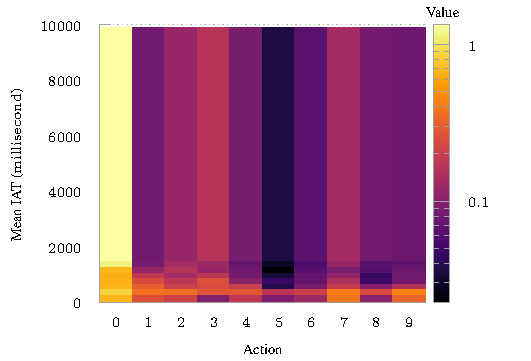
\includegraphics[width=0.9\linewidth]{../plots/policy-16-tcp-f5-mean-log}
%	
%	\caption{
%		Mean Marl action values from pre-training on mean IATs ($n=16$).
%		As these are mean values, lighter cells in each row indicate actions \emph{likely} to be taken by an agent's policy.
%		Repeated values originate from the bias tile, which is always active, and indicate regions of the state-space which have yet to be visited---here, this is most of the state space.
%		Agents visibly learn action values for tiles which override the default bias tile's preferences.
%		The measured effectiveness of this feature then suggests that a low-resolution coding over the standard region may, in fact, be a better choice.
%		We see that agents prefer to choose $p=0.0$ in most states, but higher $p$ when IATs are particularly small.
%		\label{fig:intern-16-tcp-iat}
%	}
%\end{figure}
%
%\begin{figure}
%	\centering
%	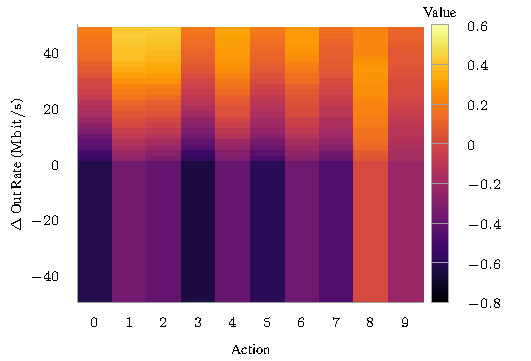
\includegraphics[width=0.9\linewidth]{../plots/policy-4-tcp-f7-mean}
%	
%	\caption{
%		Mean Marl action values from pre-training on $\Delta$ out rates ($n=4$).
%		A sudden ramp-up of server-to-host traffic is used as a strong indicator of flow legitimacy, while more punishing actions have comparatively higher value as $\Delta$ out rate decreases.
%		Furthermore, we see again that a region of the state space has gone somewhat unexplored---we observed after plotting this visualisation that many decreases in this feature are too small to hit the adjacent tile, which implies a mixed-resolution coding may improve an agent's policy further.
%		\label{fig:intern-16-tcp-something}
%	}
%\end{figure}

%?? Is the state space interpretable? Yes!
Machine learning algorithms have earned a reputation for eluding human interpretation, while being vulnerable to evasion and poisoning.
Given the security risks associated with introducing such techniques, it is natural to be concerned with the interpretability of the models we have proposed.
With the exception of global state, the tile coding parameters we make use of ensure that the set of outputs for each feature we add is relatively enumerable: for $n$ tilings and $c$ tiles per dimension there are $nc^{\dim{f}}$ individual action value vectors per feature $f$ (\num{48} for the new features we introduce, \num{10368} for global state), though considerably more combinations thereof ($c^{n \cdot \dim{f}}$).
%\Cref{fig:intern-16-tcp-iat,fig:intern-16-tcp-something} show how we may visualise the portion of a policy for each feature, and describe what information can be gained from doing so.
Furthermore, system state which is dependent on many signals drawn from across a wide network (such as our global state) is difficult to exert precise control over.
These signals' topological separation, in concert with their burstiness and unpredictability, may have substantial effects on an attacker's capabilities.

\fakepara{Real-world Deployment}
Currently, we assume that switches support an extension to OpenFlow to enable remotely installable packet-drop rules, either by running a modified version of OVS on commodity hardware at these locations or through custom firmware for egress switches.
Similar functionality could be employed by making use of OpenFlow's meter rules.

Where overheads are concerned, the state space sizes guarantee that an \emph{Instant} agent's policy remains under \SI{520}{\kibi\byte}, although in practice our sparse representation typically leads to far smaller policies: $\sim$\SI{17.8}{\kibi\byte} from our experiments.
\emph{Guarded} policies are \SI{30}{\percent} of this size.
As we have described earlier, action updates require a constant number of floating point operations---\num{160} floating point additions and \num{32} multiplications per update of $\wvec{}$ with per-tile updates, above the \num{160} additions required to choose an action.
The vast majority of these operations can be vectorised trivially, if such hardware is present.
Action computation for \emph{Guarded} agents is cheaper still, requiring only \num{48} additions per action.
Beyond this, we require that egress switches are capable of co-hosting an agent (i.e., through \emph{network function virtualisation}), with the necessary hardware to support this.
We believe that it may be possible to implement similar behaviour on standard commodity switches through application of \emph{programmable data planes} \cite{DBLP:conf/ancs/JouetP17}.

%?? Incorrect, pickling...
%?? deployment/system guidelines, architecture, and overhead/footprint of doing this
%?? Mention: probably fewer state measurements than in our emulations, but longer measurements means less noisy (so probably more accurate)
Gathering and transmission of load/flow statistics would be difficult to perform as often as an emulated environment allows, without inadvertently affecting host traffic.
However, the measurements acquired in such a scenario are likely to be less noisy (by being collected over longer periods of time), which could aid training.
The main bottlenecks are likely in forwarding the load measurements from various aggregation points (which can be made more efficient through multicast) and in running some estimator $\operatorname{g}(\cdot)$ to condition the reward function.
%?? Potential for dividing up pre-feature training across different agents, or train like this locally (sets of flows trained by 1 sub-model).
%?? Different global state per-agent? Seems this must be locally trained, just make it (everything up the chain to key destinations).
We expect that agents will be able to share policies for all features, which may help to offset the reduced rate of incoming experience.
Regardless, it will take longer to achieve enough state-state transitions to converge on a good policy.

One limit of SDN-capable hardware is that OpenFlow rules occupy \SI{6}{$\! \times$} the space of standard rules---commercial switches only have TCAM space for \numrange{2000}{20000} rules \cite{DBLP:journals/comsur/NguyenSBT16}.
Our approach consumes a rule for each active flow (the host density), and by the end of an experiment a switch can accrue around \num{900} rules.
While we use a default fallback action to maintain connectivity, eviction of high-value decisions which filter high-bandwidth attackers poses a significant risk.
Given that most flows are small (with the majority of bytes coming from a few ``heavy-hitters'') \cite{DBLP:journals/ccr/PanBPS03}, it may suffice to only apply RL-based analysis to larger flows.
%?? What could we do in the meantime? I propose manually assigning elephant flows a high importance rule, while increasing the importance of "block" decisions even higher.
OpenFlow rules have an \emph{importance}, controlling which rules may be evicted by a new entry (preventing entries from evicting those with higher importance).
If an agent is to act on all flows, a solution is to assign an importance of 0 to mice flows, 1 to elephant flows, and 2 to total filtering (leaving agents to time out and remove elephant flow rules to prevent bloat).
Given the high churn and prevalence of mice flows, eviction here is most likely to affect flows which are complete.
In both cases, extra rules can be made available by upgrading rules which completely filter a flow into upstream blackholing (as in collaborative approaches \cite{DBLP:conf/acsac/RamanathanMYZ18}), having the agent remove this rule once blackholing is active.

\section{Related Work}\label{sec:related-work}
%?? Try and compare my work here when possible?

\fakepara{DDoS Prevention}
\Textcite{DBLP:conf/lcn/BragaMP10} examine the detection of flooding DDoS attacks through \emph{self-organising maps}, using SDN to gather statistics effectively.
Many of their features aren't overly relevant, as their focus is not active defence or discovering \emph{which} hosts contribute to an attack.
%?? Actually talk about Marl (???) to appease reviewer \#1.
The closest available approach within this field is that of \textcite{DBLP:journals/eaai/MalialisK15} (whom we have positioned our work against), and their contribution in applying RL to the task of intrusion prevention is significant: their work helps to show the viability of live, adaptive, feedback-loop-like control of the network to detect and prevent DDoS attacks.
They create a tree overlay topology (subdivided into teams), where each agent applies packet drop to \emph{all} flows inbound to a protected server.
%?? Recap their flaws, since they've been cut form every other aspect.
Our results show that their technique underperforms at high host density and when congestion-aware traffic dominates---that their results do not demonstrate this suggests an evaluation driven purely by traces (rather than live application dynamics).

\emph{SPIFFY} \cite{DBLP:conf/ndss/KangGS16} aims to remedy transit-link attacks by observing how flows from each source respond to a sudden increase in available bandwidth.
\Citeauthor{DBLP:conf/ndss/KangGS16} realise that bots participating in an attack are often unable to match this bandwidth expansion (having already saturated the capacity of their outbound links), while legitimate flows typically speed up to match the new fair-share rate.
%Attackers must either be detected or reduce the throughput of each bot, increasing the cost of launching an attack.
%Unlike our approach (and due to the class of attacks it is designed to defend against), SPIFFY is intended to be deployed within ASes, although .
A weakness of their approach is that computing a route to measure bandwidth expansion on real networks can be costly (up to \SI{14}{\second} for the Cogent topology), and that the low expansion factors in real network can require more ``rounds'' of filtering.
By contrast, our approach takes a constant time to compute an action for a flow regardless of topology size.
Their assumptions about traffic response to such bandwidth expansion do not hold for constant bitrate flows (e.g., VoIP) and may not extend to HTTP DASH flows, both of which make up a sizeable proportion of network traffic.

\emph{Athena} \cite{DBLP:conf/dsn/LeeKSPY17} is a generalised SDN framework for intrusion detection, but has shown the use of a \emph{k-nearest neighbours} classifier to detect individual attack flows.
Although heavyweight (and proven to be effective compared with \textcite{DBLP:conf/lcn/BragaMP10}), their comparison against SPIFFY lacks the quantitative evidence required to understand how the system compares.
\Textcite{DBLP:conf/sp/SmithS18} use AS-level routing to tackle both transit-link and flooding-based attacks.
This view is taken due to the perceived cost of per-stream classification and inherent sensitivity to adversarial examples.
The approach is creative, relying upon BGP \emph{fraudulent route reverse poisoning} to preserve traffic to a target AS, but unlike SPIFFY the approach doesn't actually \emph{remove} the congestion.
Because of this, flooding-based attacks aren't fully alleviated.

%?? Abuses of RL 
\fakepara{RL in Networks}
Earnest, well-considered application of RL towards the challenge of intrusion prevention has seen comparatively little examination.
Past work treats the paradigm as a traditional classifier for anomaly detection \cite{shamshirband2014anomaly} and DDoS prevention \cite{DBLP:conf/mates/ServinK08}.
Given that the main strengths of RL techniques are the ability to control ongoing interaction and adapt by observing the concrete effects of actions, such works don't apply the rich literature on the subject to its fullest potential.

For categorising how RL fits into solving problems, we label works as direct- or indirect-control RL.
A \emph{direct-control} RL problem is one where the RL agent(s) learn optimal control over a set of actions as the \emph{primary} defence or decision-maker---requiring measurements, reward functions and action sets tailored for this purpose.
%We feel there is a shortage of work in this category at present, at least in the field of networks.
To date, the best-fitting example we have encountered is that of \textcite{DBLP:journals/eaai/MalialisK15}.
An \emph{indirect-control} RL problem is one where agents act in service to \emph{another technique} responsible for decision-making, optimising or generalising aspects of its operation beyond that of hand-coded heuristics.
A past example includes learning when best to share knowledge between \emph{hidden Markov model} anomaly detectors \cite{DBLP:conf/paisi/XuSH07}.
%The position of this work is weakened by its reliance on the problematic `DARPA99' dataset \cite{DARPA-IDD, DBLP:conf/cisda/TavallaeeBLG09, DBLP:conf/sp/SommerP10}, but the idea itself is well-treated and this acts as a driver for improvements in this direction.
This work is weakened by its reliance on the problematic `DARPA99' dataset \cite{DBLP:conf/sp/SommerP10}, but the idea itself is well-treated.
Outside of intrusion detection, there has been growing interest in the use of RL in data-driven networking, such as for intra-AS route optimisation \cite{DBLP:conf/hotnets/ValadarskySST17} and resource-constrained process allocation \cite{DBLP:conf/hotnets/MaoAMK16}.
\textcite{DBLP:conf/sigcomm/MaoNA17} employ client-side observations of network state and video performance with RL to optimise bitrate selection for multimedia streaming.
\emph{AuTO} \cite{DBLP:conf/sigcomm/ChenL0L18} employs deep RL to perform traffic optimisation.
Crucially, they find that the vast majority of flows are short-lived, requiring effective decisions in less than a millisecond.
To overcome the high latency of action computation via a neural network, two agents are trained, handling aspects of short and long flows respectively.
The first learns to optimise the flow size thresholds to demarcate long and short flows; these short flows are routed by ECMP.
The second agent makes bespoke decisions about routing, prioritisation etc.\ for each of the remaining long flows.


\section{Conclusions and Future Work}
Through this paper, we have discussed reinforcement learning and its relevance to network intrusion prevention.
We believe the potential to learn feedback loop-like control online and against non-stationarity makes it particularly suited to the problems endemic to the field.
We identified weaknesses in past work, recommending an RL agent which acts per flow, and have outlined the algorithmic and engineering choices needed to make its deployment feasible.
Supporting this, we've presented an in-depth examination of our feature space, offering quantitative and qualitative justification for our choices.
Our evaluation shows that our new agent designs considerably advance the state-of-the-art in RL-based DDoS prevention, with \emph{Guarded} agents showing the most promise for future evaluation.

The most direct improvements to be made lie in the correct protection of legitimate UDP traffic, which our agent designs have difficulty safeguarding.
Outside of this, there is scope to test these new techniques against link-flooding attacks in large-scale topologies using reward functions such as \cref{eqn:lfa-reward}.
Simulation is the most likely avenue for such evaluation.

%(rather than na\"{i}ve simulation, blind ML applications etc.) and choose well-considered pathways to solution. \emph{Call-to-action}?

%\section{Future Work}
%Airlift half of the ``conclusion'' and paste it in here, so that it can be a lot neater.
%?? Future Work? I.e., \emph{everything}: no one else is really looking at/interested in this specific kind of application of RL yet. \emph{Yet}.

%?? IDEA: try out average reward, TD($\lambda$) methods as future work...
%A natural research direction to enhance this work would be the combination of the classic function approximation techniques we make use of alongside the improved algorithms that the RL community has introduced in the past few years.
%Actor-critic methods, or algorithms based on eligibility traces are good candidates for investigation. 
The remaining weaknesses invite many improvements worth investigation.
%?? What might we do for a reward function in the absence of heuristic estimates and/or explicit a priori knowledge? I think a good candidate is the sum of up and down throughputs (normalised by capacity sum), so long as \emph{neither exceeds the link capacity}. We can extend the team-based formulations similarly. This, in theory, promotes traffic diversity since it's not like flooding-based DDoS attacks are going to submit meaningful work to a server. The intuition, I suppose, is that certain classes of flow will have a small footprint in one direction which causes a sizeable increase in the other! Alternatively, monitor the health of canary flows which cross the team boundary (i.e. only one in-out link).
A problem we raised (without a clear solution) was the design of reward functions which do not rely upon heuristic estimates or a priori knowledge of benign traffic content.
If true online learning is desired (i.e., coping with a non-stationary environment), then such reward functions are sorely needed.
While $\bload{\cdot}$ is likely to be a good candidate for many deployments, we believe that finding an effective metric derived from the individual statistics we suggested serves as an interesting research problem.

%?? Benefit of the more realistic emulation environment is that it is far closer in behaviour and architecture (i.e. viable) to a real SDN-enabled deployment, captures some dynamics which were otherwise hidden/lost by human ignorance. It also allows me to develop the system towards evolving traffic models where it is expected that RL should shine over and above standard ML techniques. THEN: Room to introduce/roll-in dynamic changepoint detection or adaptive exploration \cite{DBLP:conf/ki/Tokic10, DBLP:conf/ki/TokicP11, DBLP:conf/annpr/TokicP12}?
Given that one of the advantages of RL methods is the ability to handle non-stationary problems, it is important to propose and test sensible simulations or captures of evolving networks.
While it is known that DDoS attack strategies evolve in real time \cite{DBLP:conf/spw/KangGS16}, evaluation is difficult at present since no works detail what patterns such evolution might take.
Regardless, these scenarios present ideal circumstances to apply adaptive exploration \cite{DBLP:conf/annpr/TokicP12}, changepoint detection, or intelligent sampling methods to judge which flows are most worthy of consideration.
For estimating \emph{when} to explore, we believe that the intersection of signal processing and RL is as-yet unexplored.

%?? IDEA: Apply these techniques to programmable data planes etc. While it's pretty neat that what we have works assuming that ach router is a software (x86) switch running OVS, what might we need to consider when applying this to `real' switches? ``PDP can allow this to be added to real routers to make it efficient to keep \& process state in the manner we require, as well as enabling more adaptive deployment''. Cite P4, BPFabric, other work on PDPs?
%?? What concessions will we have to make in order to make per-flow processing more viable? Intelligent sampling/reanalysis of flows when needed (i.e. an external heuristic guiding method)? In SPIFFY's \cite{DBLP:conf/ndss/KangGS16} evaluation, we see clearly that it can take around \SI{2}{\second} for a flow to react fully to a rate increase---I think for the TCP step it may be wise to factor this in, too!
%?? More future work --- share knowledge between agents. ``Knowledge bases'' for this purpose? (see: Qianru).
Effective real-world deployment of RL-based defences cannot assume that switches in a network will support a custom version of OVS or other arbitrary software, introducing the question of whether agent training, execution and distribution may be possible when using \emph{programmable data planes} \cite{DBLP:conf/ancs/JouetP17}.
We also expect it will be fruitful to look into \emph{how} agents may share knowledge with one another.

%?? Security? I suspect that the very qualities that make inference difficult in IDS/IPS also increase the level of challenge an advanced threat must overcome.
%?? Might want to mention it in related work above, but the recent attention on adversarial examples/tricking models needs to be looked into for RL. Poisoning attacks relevant for online techniques: old bounds exist \textcite{DBLP:journals/jmlr/KloftL10}, new stuff concerns collaborative learners \cite{DBLP:conf/acsac/ShenTS16}, nothing for rl. Hot topic in deep networks \cite{DBLP:conf/eurosp/PapernotMJFCS16, DBLP:conf/eurosp/PapernotMSW18}, but naturally still relevant with even linear approximations or exact tabular case due to limits of the PAC assumption. There is now examination of evasion attacks wrt.\ RL \cite{DBLP:journals/corr/HuangPGDA17}!
%?? evasion attacks by \textcite{DBLP:conf/sp/Carlini017}---all of these are computed by way of a general stochastic optimiser, such as \emph{Adam} \cite{DBLP:journals/corr/KingmaB14}. possible to apply something similar to our learned model to assess its security? would the suggested states even be valid? (i.e. since they're monotonically increasing for the most part).
Although we believe that the security landscape for classical RL models is not \emph{identical} to that of neural-network based approaches (particularly with such noisy, volatile, and hard-to-control data), there is still immense value in determining the exact capabilities of a sufficiently powerful adversary as the risk of external control still exists.
In particular, we believe that poisoning attacks and evasion attacks merit close consideration.

%While this work still trails behind the performance of exact DDoS flow detection mechanisms, w
We hope it is clear that reinforcement learning holds promise and can inspire further innovation.
It allows us to offer distinct advantages above existing works, such as protocol-agnostic DDoS flow detection, flexible deployment, and automatically learned low-overhead decision-making---without requiring many of the 
network resources or capabilities that other techniques rely upon.
It's hoped that more research in this direction will open the door to works which \emph{respect the complexity of the network}; evolving topologies, natural change in traffic and protocol distributions, and the mutation of attacks.

